\documentclass[12pt, a4paper]{report}
\author{oslo@itu.dk&ppho@itu.dk}
\usepackage[english]{babel}
\usepackage[utf8]{inputenc}
\usepackage[T1]{fontenc}
\usepackage{lmodern}
\usepackage{graphicx}
\usepackage{appendix}
%\usepackage[left=3.5cm,right=3.5cm,top=3.3cm,bottom=3.3cm,heightrounded]{geometry} %MS Word kind of margins
\usepackage{geometry}
\usepackage{amsmath}
\usepackage[numbib,nottoc]{tocbibind} % nottoc removes Contents reference in toc
\usepackage{titlesec, blindtext}
\usepackage{csquotes}
\usepackage{pdfpages}
\usepackage{epsfig}
\usepackage{epstopdf}
\usepackage{framed, color}
\usepackage{xcolor,colortbl}
\usepackage{enumerate}
\usepackage{booktabs}
\usepackage{tabularx}
%\usepackage{natbib}
%\bibliographystyle{abbrvnat}
%\setcitestyle{authoryear,open={(},close={)}}
\usepackage{microtype}
\usepackage[backend=biber,style=apa,natbib=true,url=true]{biblatex}
\DeclareLanguageMapping{english}{british-apa}
\usepackage[bookmarks,hidelinks]{hyperref}
\usepackage[colorinlistoftodos]{todonotes} %Margin todo notes and comments
%\todo{Plain todonotes.} - add a '%' on the end for a line to the position in text
%\todo[color=blue!40]{Todonote with a different color.}
%\todo[nolist]{Todonote that is only shown in the margin and not in the list of todos.}
%\todo[inline]{testing testing}
%The command: \listoftodos - This is for rendering a list of todos
%\setlength{\emergencystretch}{3em} %Accept a little stretch in order to fit lines

\usepackage{array}
% A left-aligned column with a set width (L{3cm}).
\newcolumntype{L}[1]{>{\raggedright\let\newline\\\arraybackslash\hspace{0pt}}m{#1}}
% A center-aligned column with a set width (C{3cm}).
\newcolumntype{C}[1]{>{\centering\let\newline\\\arraybackslash\hspace{0pt}}m{#1}}
% A right-aligned column with a set width (R{3cm}).
\newcolumntype{R}[1]{>{\raggedleft\let\newline\\\arraybackslash\hspace{0pt}}m{#1}}

%COLORS
\definecolor{undonecolor}{rgb}{1,0.6,0.6} %Comment/undone color
\definecolor{shadecolor}{rgb}{0.9,0.9,0.9} %Use Case background
%COLORS

%REFS
%\bibliographystyle{IEEEtran}
%\bibliography{IEEEabrv,references.bib}
%\bibliography{mendeley.bib}
\addbibresource{VRHandsThesis.bib}
%REFS

\DeclareSourcemap{
    \maps{
        \map{ % Replaces '{\_}', '{_}' or '\_' with just '_'
            \step[fieldsource=url,
                  match=\regexp{\{\\\_\}|\{\_\}|\\\_},
                  replace=\regexp{\_}]
        }
        \map{ % Replaces '{\#}', '{#}' or '\#' with just '#'
            \step[fieldsource=url,
                  match=\regexp{\{\\\#\}|\{\#\}|\\\#},
                  replace=\regexp{\#}]
        }
        \map{ % Replaces '{'$\sim$'}', '$\sim$' or '{~}' with just '~'
            \step[fieldsource=url,
                  match=\regexp{\{\$\\sim\$\}|\{\~\}|\$\\sim\$},
                  replace=\regexp{\~}]
        }
    }
}

%TABLE POSITIONING
\usepackage{float}
\restylefloat{table}
%TABLE POSITIONING

% CHAPTER FORMATTING
\definecolor{gray75}{gray}{0.75}
\newcommand{\hsp}{\hspace{20pt}}
\titleformat{\chapter}[hang]{\Huge\bfseries}{\thechapter\hsp\textcolor{gray75}{|}\hsp}{0pt}{\Huge\bfseries}
\titlespacing*{\chapter}{0pt}{0pt}{40pt}
% CHAPTER FORMATTING

\renewcommand{\arraystretch}{1.5}

% COMMENTING
\newcommand{\comment}[1]{\colorbox{undonecolor}{#1}}
% COMMENTING

% COMPACTING LISTS
\newenvironment{packed_itemize}{
\begin{itemize}
  \setlength{\itemsep}{3pt}
  \setlength{\parskip}{0pt}
  \setlength{\parsep}{0pt}
}{\end{itemize}}
% COMPACTING LISTS

\setcounter{secnumdepth}{0} % sections are level 1

% Set base path for images.
\graphicspath{ {Images/} }


\begin{document}

% Set sans serif font family.
\sffamily

% Include the ITU frontpage!
%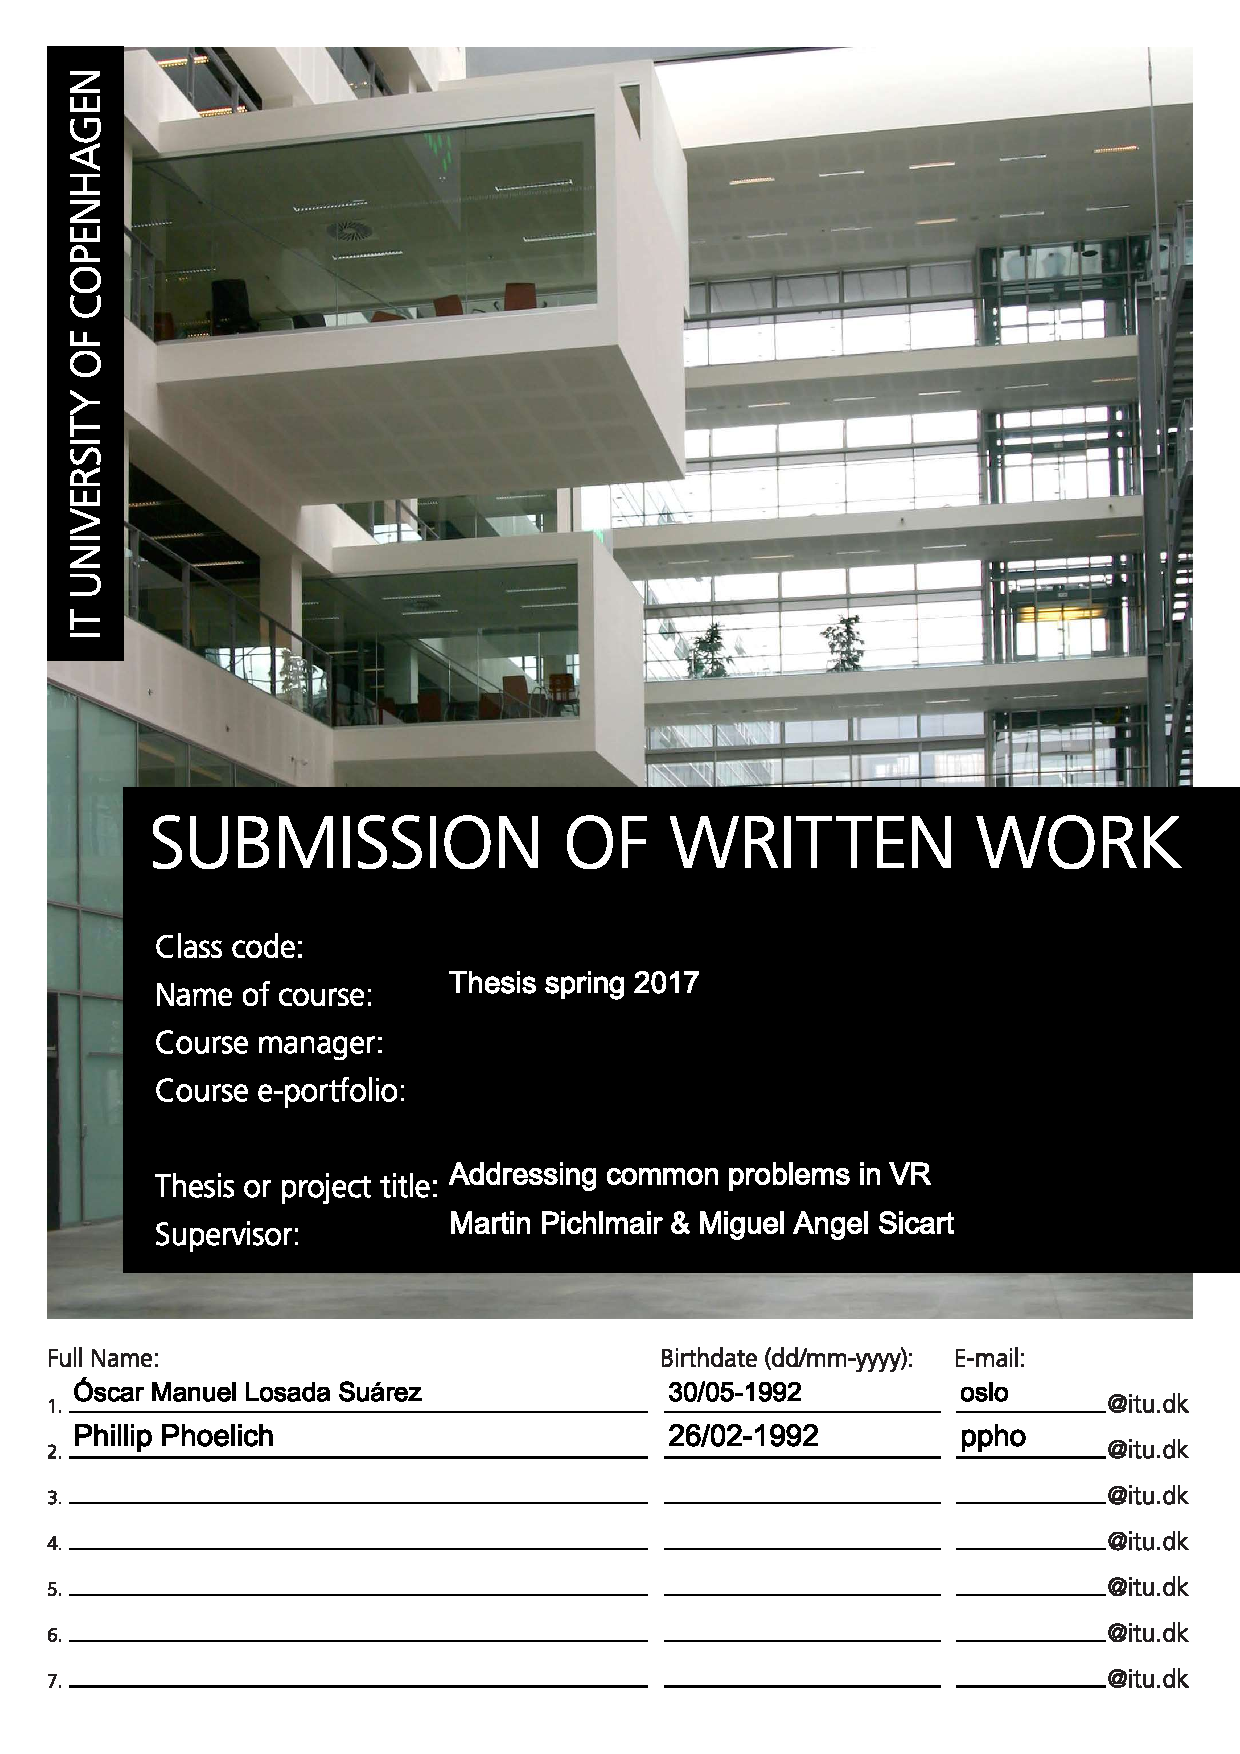
\includepdf{ITUfrontpage.pdf}

\listoftodos

% TITLEPAGE
\newgeometry{left=0.1cm,right=0.1cm}
\begin{titlepage}
\begin{center}

\textsc{\large Thesis paper}\\[2cm]

\textsc{\huge \textbf{Hands in Virtual Reality}}\\[8.2cm]
%\textsc{\large \textbf{With a focus on embodiement and the player's intensions}}\\[2cm]

\textit{Authors}\\
Óscar Manuel Losada Suárez\textit{(oslo@itu.dk)}\\
Phillip Phoelich \textit{(ppho@itu.dk)}\\[1cm]

\textit{Supervisors}\\
Martin Pichlmair\\
Miguel Sicart\\[1cm]

\textit{Date}\\
June 1st, 2017\\

\vfill
\textit{MSc in Games}\\
\textsc{IT University of Copenhagen}

\end{center}
\end{titlepage}

\restoregeometry

% ABSTRACT
\begin{abstract}
Here is the abstract of the thesis paper.
\end{abstract}

% TABLE OF CONTENTS
\tableofcontents
\newpage


%MAIN CONTENT
\newgeometry{top=3.9cm}

\chapter{Introduction}
\label{chap:introduction}
In our day-to-day lives, we constantly use our hands to hold, operate and otherwise manipulate objects, tools and devices with precision. We use them to gather tactile information about the world and even to communicate with each other through hand gestures and body language. They are a fundamental part of the human body and our way of interacting with the world around us.

The biggest buzzwords in the Virtual Reality (VR) medium: immersion and presence, perhaps point us in the right direction. VR is meant to bring us closer than ever before to experiencing virtual environments as if we were actually in them. Interaction is a big part of experiencing the places we are in. It should hardly be a point of contention then, that having virtual hands that imitate our own real hands can have a significant impact on VR experiences.

VR game developers and hardware manufactures alike have acknowledged this. Major consumer-oriented VR devices like the HTC Vive, the PlayStation VR  with the PlayStation Move Motion Controllers (PS VR + Move) and the Oculus Rift + Touch have controllers that track the position of your hands in space \parencite{htcvive2016, psvr2016, psmove2010, oculus2016}. In their About page, Owlchemy Labs, the creators of the critically and commercially acclaimed \parencite{UnityAwards2016, SteamSpyJobSim} Job Simulator: the 2050 archives \parencite{OwlchemyLabs2016} declare:

\begin{displayquote}
\textit{We believe that interaction and using your hands is what truly makes virtual reality the most incredible place to build unique content that blows players minds.} \parencite{aboutOwlchemyLabs}
\end{displayquote}

Predictably enough, this is not the end of the story. Even if we had complete tracking of the hands and individual fingers, the physical constraints of the virtual environment would still not apply to the users' real hands, which leaves us with few essentially different options:

\begin{enumerate}
\item Prioritize user input and ignore virtual environment constraints whenever there is a conflict in order to always keep the virtual hands aligned with the real hands to the extent allowed by the tracking data.
\item Separate the virtual hands from the real hands when there is conflict in order to respect the virtual environment's constraints.
\item Use sensory feedback that makes the users either respect the virtual constraints on their own or feel like they are constrained without actually being so.
\item As \parencite{Schell2015} suggests, design in a way that circumvents the problem, which means restricting the medium's content to experiences that fit exactly to the medium's current affordances \parencite{Norman}. This means seeing limitations as features and finding experiences that map perfectly to the current systems.
\end{enumerate}

The work here presented is focused on the second option, which is seen as a directly opposite alternative to the first. We aim to explore how virtual hands can work in this case and investigate whether the user experience can be improved with this approach.

From this point on, we will refer to this problem as the Virtual Constraints Problem, to the approaches fitting the first option as Unadjusted Hand Control Models and to those fitting the second option as Adjusted Hand Control Models.

\begin{figure}[h]
\centering
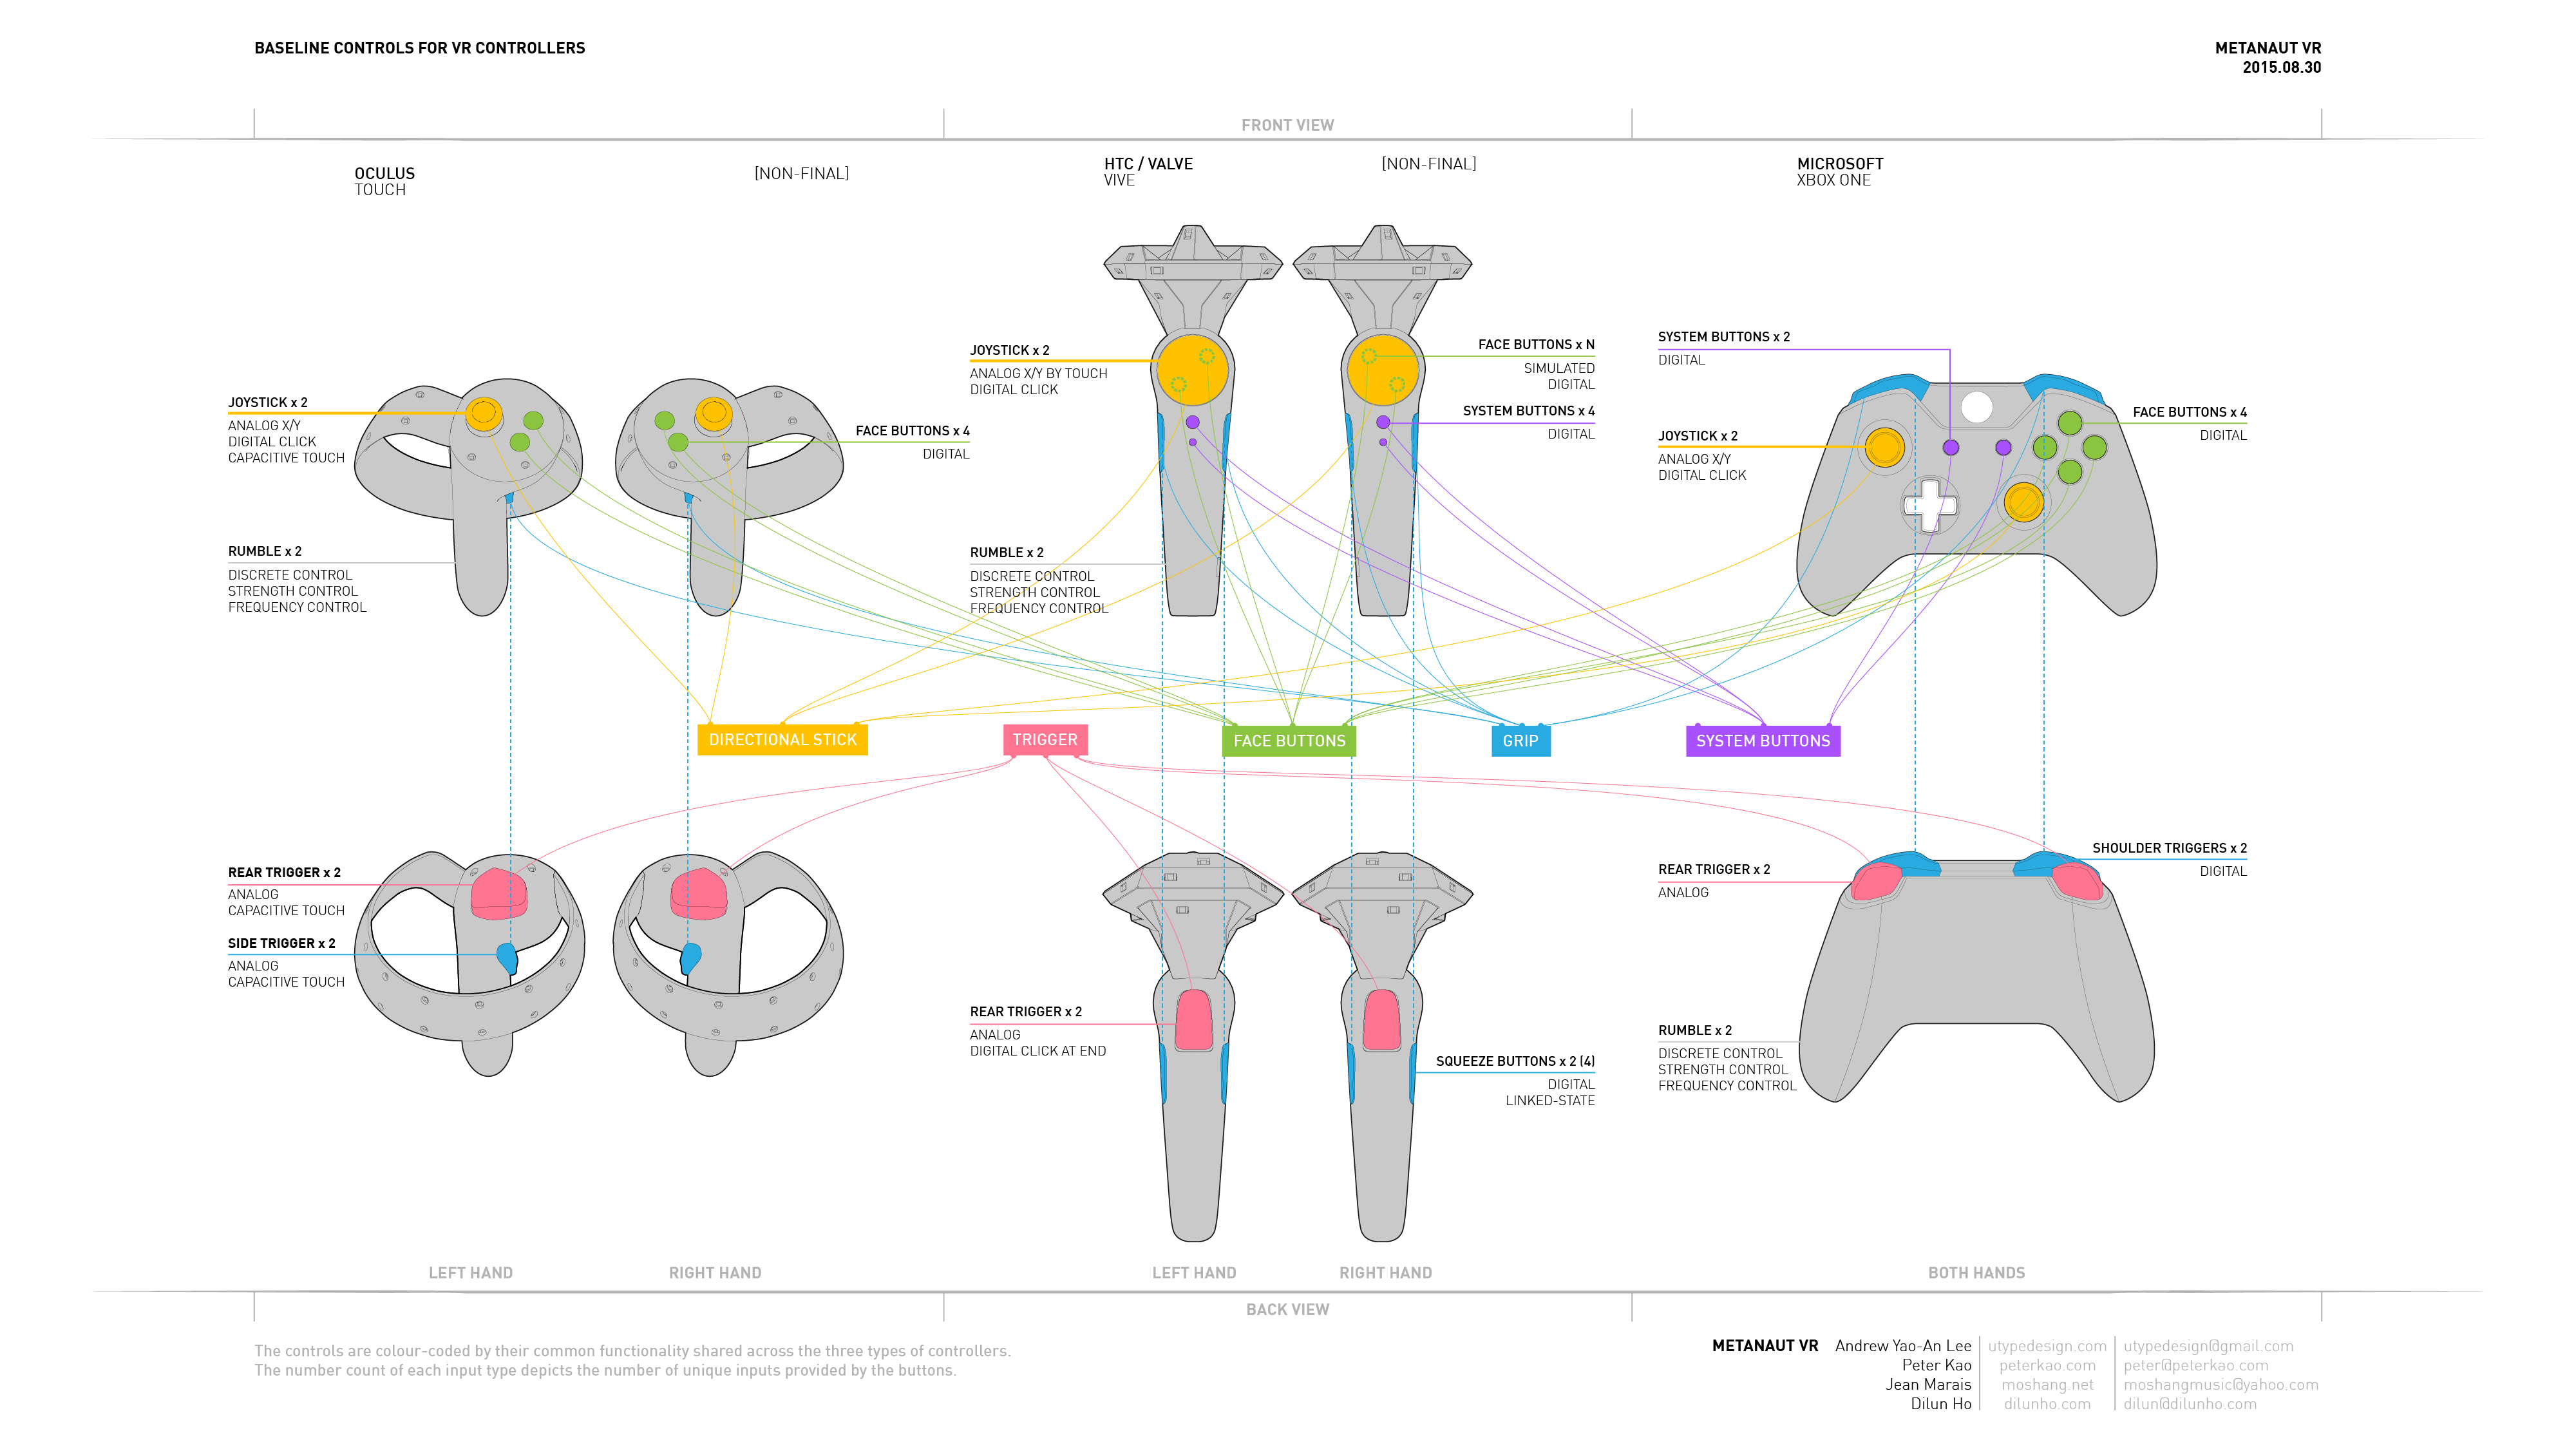
\includegraphics[width=\textwidth]{vrcontrollersbaselinecomparison2c.png}
\caption{Comparison of VR controllers and their different input and output capabilities. Note that the final version of the HTC Vive controllers looks different. Retrieved from\parencite{MetanautVR2015} and can be seen in a larger format in Appendix \ref{apx:vrControllerComparison}.}
\label{fig:vrControllerComparison}
\end{figure}

\section{State of the Art}
\label{sec:stateOfTheArt}

\subsection{VR Hardware}
\label{subsec:vrHardware}

There is a considerable amount of devices and accesories that are relevant to VR. This work is mainly applicable to those setups that can spatially track the hands of the user to a similar or greater degree than the HTC Vive allows. We are particularly interested in findings that are relevant to the aforementioned HTC Vive, PS VR + Move and the Oculus Rift + Touch because they are currently the most important consumer-oriented devices with these capabilities \parencite{Armstrong2017, SuperDataLLC2017}.



There are differences between the Head Mounted Displays (HMD) of these devices, but for the most part, they are not relevant for our area of focus, so they will not be discussed here.

On the other hand, it might be worth briefly covering the differences in terms of spacial tracking of the controllers between the devices. The HTC Vive allows 360 degree tracking within the biggest space volume, the Oculus Rift + Touch with the default setup is designed mainly for 180 degree tracking, but an experimental setup with extra components allows stable 360 tracking \parencite{Lang2016, Kuchera2016}.

Figure \ref{fig:vrControllerComparison} shows the features of the Oculus Touch and the HTC Vive controllers. In the case of the HTC Vive, the most relevant features for our purposes are:

\begin{itemize}
\item the analogue triggers with digital click at the end, controlled with the index finger, 
\item the digital grip buttons, pressed with middle, ring and/or pinky fingers,
\item the joysticks or trackpads, with analog x/y input through capacitive touch and digital click, used with the thumbs
\item and rumble capabilities.
\end{itemize}

In the case of the Oculus Touch, the relevant features are:

\begin{itemize}
\item the analogue triggers with capacitive touch, controlled with the index fingers, 
\item the analogue side triggers, pressed with middle, ring and/or pinky fingers,
\item the joysticks, with analog x/y input, digital click capacitive touch, used with the thumbs
\item and rumble capabilities.
\end{itemize}

Figure \ref{fig:psmoveDiagram} shows the input mechanisms of the PS Move Motion Controller, again, the most relevant features are:

\begin{itemize}
\item the analogue T buttons, controlled with the index fingers,
\item several digital buttons controlled by the thumbs
\item and rumble capabilities.
\end{itemize}

\begin{figure}[H]
\centering
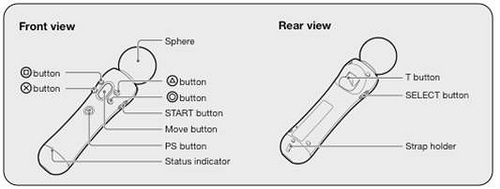
\includegraphics[width=\textwidth]{psmovecontroller.jpg}
\caption{Diagram of the PS Move Motion Controller. T button allows analogue input. Retrieved from \parencite{psmoveDiagram}.}
\label{fig:psmoveDiagram}
\end{figure}

Analogue buttons are useful to allow the users to control the motion of the virtual fingers with similar movements with their own fingers - in Norman's terms, they provide a natural mapping \parencite{Norman} for finger control. Similarly, although without the advantage of being analogue, buttons or areas with capacitive sensors can be used to monitor if the user's fingers are resting on the controller or are lifted, which can allow for guessing the position of the fingers. 

The Oculus Touch is the controller that takes these input mechanisms further having a capacitive trigger for the index finger, capacitive buttons for the thumb and a normal trigger for the other three fingers. This can be used to detect a variety of gestures like index finger pointing, thumbs up (or down), finger guns... It also facilitates common interactions like pressing virtual buttons with your virtual index finger, operating a grabbed object with the same hand that is holding it (e.g. press gun trigger). Both the HTC Vive and PS VR controllers allow for a lower degree of natural finger control.

Other accessories exist that allow for actual positional tracking of the fingers, such as the Manus VR Gloves \parencite{ManusVR2016}. These would of course enhance the experience, but ultimately would face the same problem because they don't provide a way to impose constraints from the virtual world on the real hands of the user.

\subsection{VR Games}
\label{subsec:vrGames}

The most frequent approach to dealing with the Virtual Constraints Problem described at the beginning of this chapter is to ignore these constraints when they conflict with the user input. Job Simulator is a prime example of the unadjusted hand model and the one that we have used in our work as a baseline for comparison.

In Job Simulator the hands never separate from the position of the controller, but this still allows for reasonable physical interaction with small, light objects that can be easily moved by the hands. When the hands collide with movable objects, the object is pushed out of the way. However, when the virtual hands collide with objects that cannot be moved by them, the hands will simply go through them as if they weren't there as shown in Figure \ref{fig:jobSimStaticProblem}.

\begin{figure}[H]
\centering
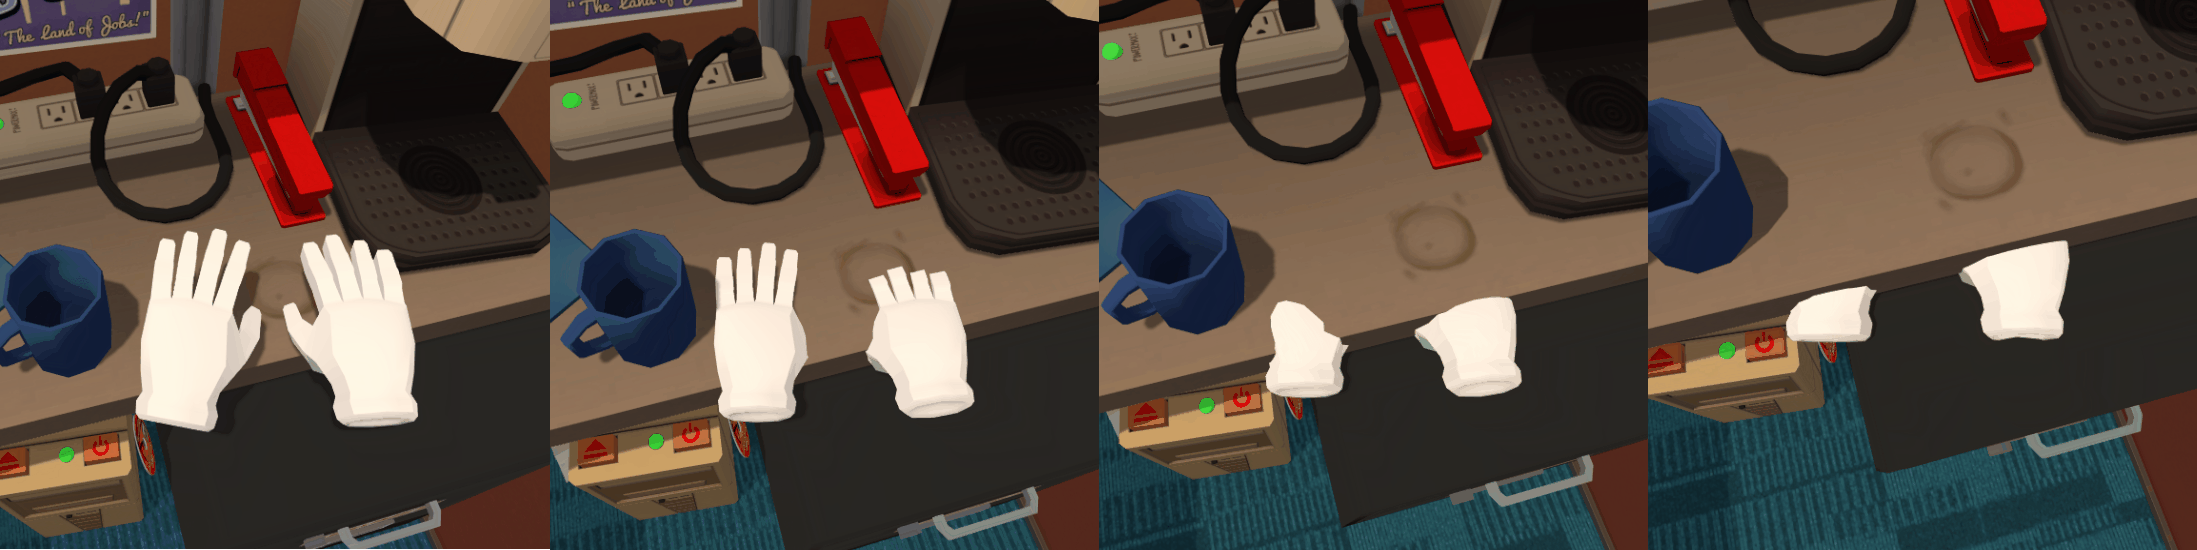
\includegraphics[width=\textwidth]{Sequences/JobSimulator/jomSimStaticProblem.png}
\caption{Sequence showing the Job Simulator hands entering an immovable obstacle. Captured in the HTC Vive version. A gif can be found here: \url{https://tinyurl.com/JobSimTouchStatic} .}
\label{fig:jobSimStaticProblem}
\end{figure}

At the same time, they avoid the problem of grabbing objects with correct finger placement by hiding the hands when they are holding an object as shown in Figure \ref{fig:jobSimGrabProblem}. This solution is not without merits: it allows the user to see the held object from all angles without the hand obstructing the view, it is simple and surprisingly, it is often not noticed by the users.

Ideally however, we would like the hand to be visible and the fingers to be correctly placed on the grabbed object forming a grip. But without adjusting the virtual hand, this requires the user to be too precise controlling the virtual hands and makes grabbing objects very difficult.

\begin{figure}[h]
\centering
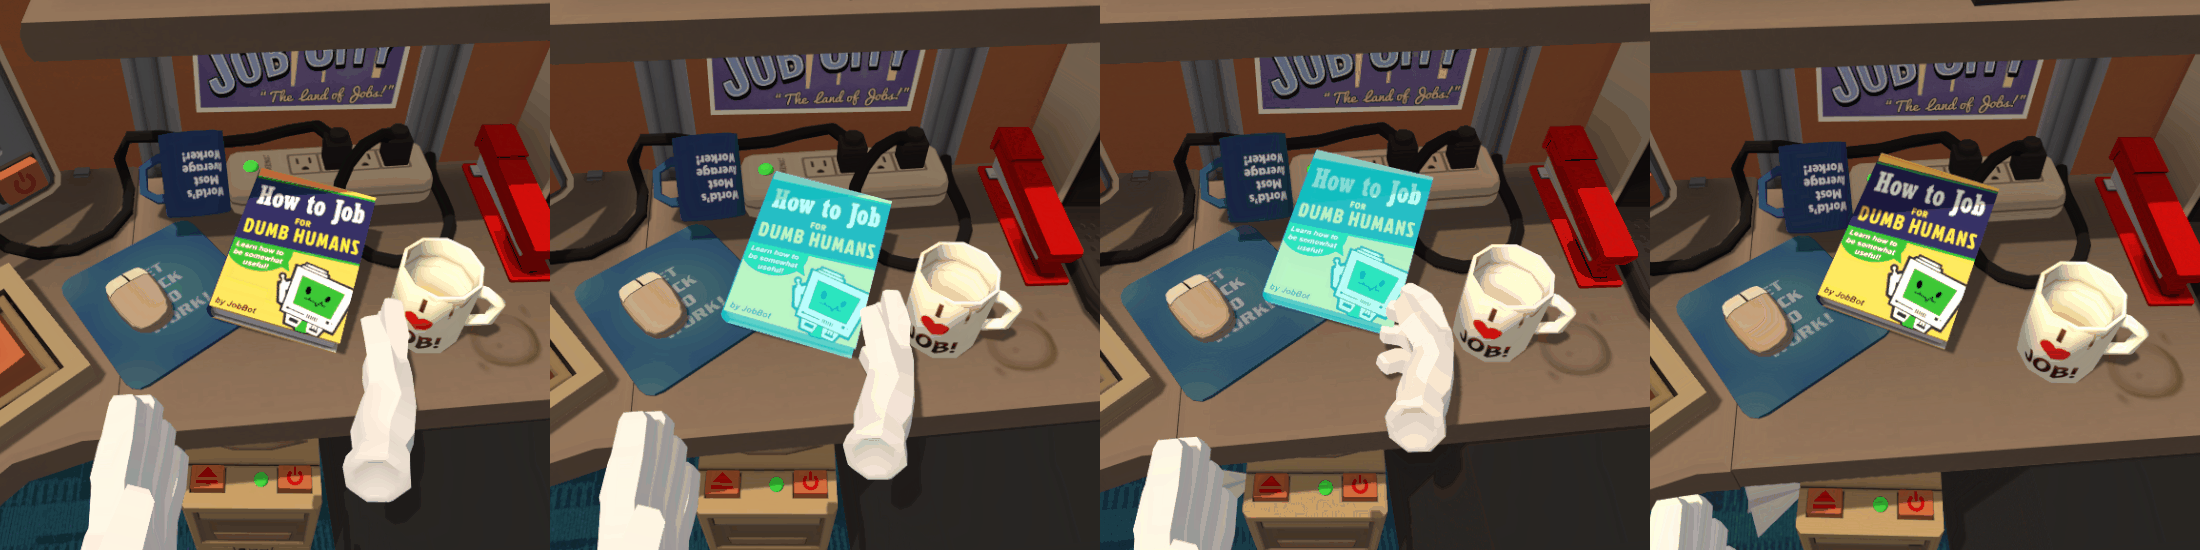
\includegraphics[width=\textwidth]{Sequences/JobSimulator/jomSimGrabProblem.png}
\caption{Sequence showing the Job Simulator hands grabbing an object. The hands are hidden while holding objects. Captured in the HTC Vive version. A gif can be found here: \url{https://tinyurl.com/JobSimGrabObject} .}
\label{fig:jobSimGrabProblem}
\end{figure}

Very recently, a few games have started to show approaches to hand control that fall within the adjusted hand model. One these is Wilson's Heart \parencite{TwistedPixelGames2017}, released in April this year. Each object that the user can interact with has a predefined hand pose and when certain conditions are met, the hands will snap to the pose as shown in Figure \ref{fig:wilsonGrab}. These conditions usually have to do with the user pressing some of the triggers or buttons that control the virtual fingers although there are also poses that are triggered by moving the hands close enough to the objects.

\begin{figure}[h]
\centering
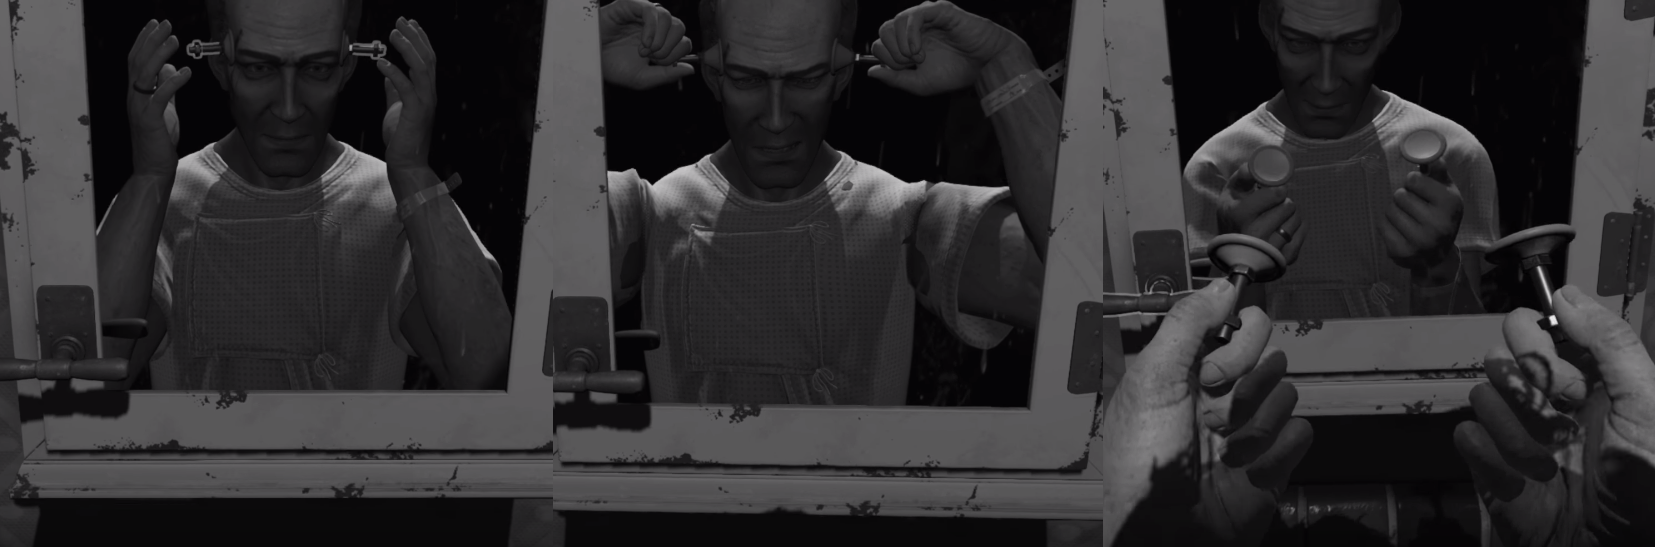
\includegraphics[width=\textwidth]{Sequences/WilsonsHeart/wilsonGrab.png}

\vspace{0.15cm}

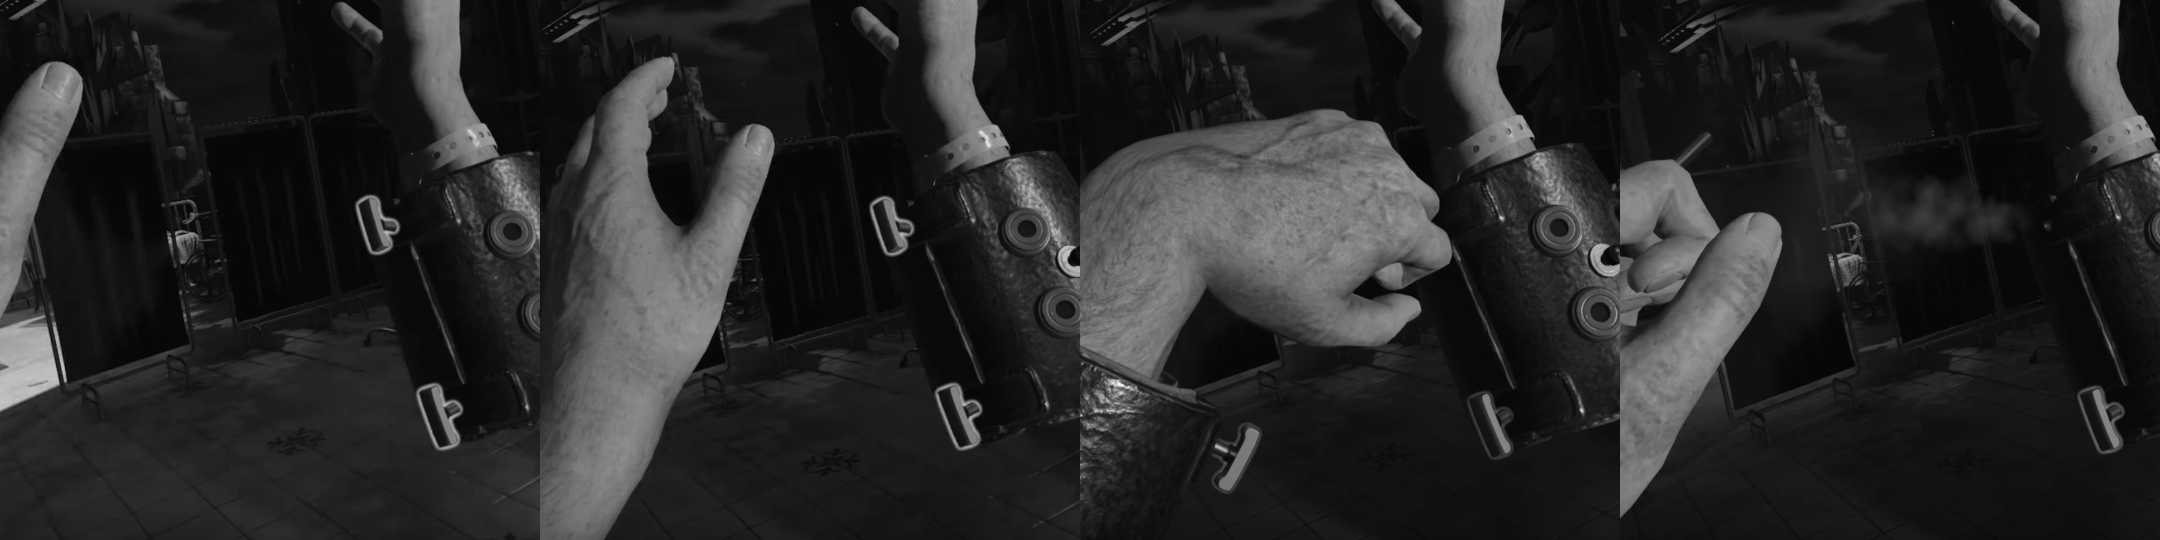
\includegraphics[width=\textwidth]{Sequences/WilsonsHeart/wilsonGrabCuffs.png}
\caption{Sequences showing the pose-snapping grab in Wilson's Heart. Two gifs showing the pose-snapping can be found here: \url{https://tinyurl.com/whGrabPoseMirror} and \url{https://tinyurl.com/whGrabPoseCuffs} .}
\label{fig:wilsonGrab}
\end{figure}

This technique is interesting because the virtual hands can separate a lot from the position of the real hands and very suddenly too. The underlying idea is that user's want to interact with each object in a certain way and will on their own pose their hands in a similar way to the object's pose, so when the pose snapping happens, the change will be small and, most importantly, aligned with the user's intention. 

The pose-snapping method allows perfect placement of the fingers and looks great in pictures, but it requires a lot of manual work to setup every interactible object in the game and it takes away a lot of control from the users, forcing them to interact with each object exactly in the ways that the poses allow.

\begin{figure}[h]
\centering
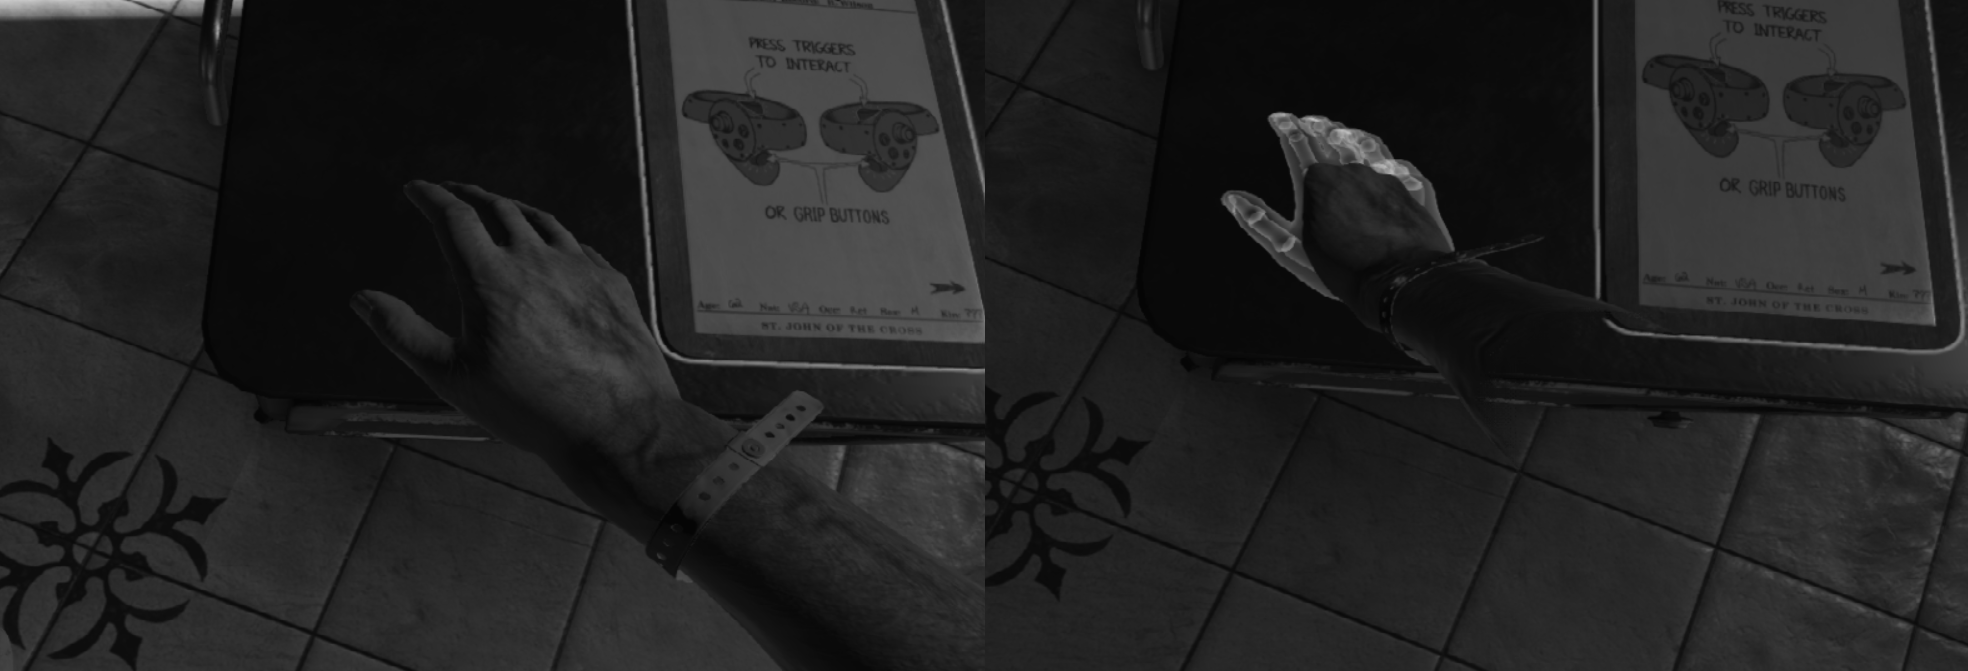
\includegraphics[width=\textwidth]{Sequences/WilsonsHeart/wilsonPenetration.png}
\caption{Sequence showing the hands in Wilson's Heart entering an immovable object. An X-Ray effect shows the part of the hand inside the object. A gif can be found here: \url{https://tinyurl.com/whPenetration} .}
\label{fig:wilsonPenetration}
\end{figure}

Figure \ref{fig:wilsonPenetration} shows that the other issue identified with the Job Simulator hands is mostly unsolved in Wilson's Heart. The hands can still go through immovable objects, but in this case, an X-Ray style effect is used to visualize the parts of the hands that are inside of objects. This communicates the state of the hands to the player, but might not be preferable to other techniques that make the virtual hands respect the virtual world's physics.

The most novel and promising attempt within the adjusted hand model that we are aware of however, is an upcoming game called Lone Echo \parencite{ReadyAtDawn}. In this game, the virtual hands procedurally adapt to the virtual environment. Once again, the underlying principle is adjusting the virtual hand in a way that doesn't conflict with the user's intentions, but in this case instead of using authored poses the use of a real-time algorithm can make the system extremely flexible. At its best, this approach could empower the user and make them feel more control over their virtual hands by not forcing the interaction with objects to one specific pose. At its worse, there might be situations where the algorithm doesn't behave in a way that matches the user's natural way of interacting with their hands which would have the opposite effect.

This approach will inevitably come at the cost of having some edge cases that don't look as good authored poses, but in terms of development work, scales much better with the amount of objects in the virtual environment and these edge cases might be so rare that they barely impact the experience.

Figure \ref{fig:loneEchoGrip} tries to show the procedural hand posing shown in some of the available footage from the game, but in this case particularly - and in general for the other frame sequences included in this work - we encourage the reader to watch the linked videos and .gifs because a few frames can't possibly do them justice.

\begin{figure}[H]
\centering
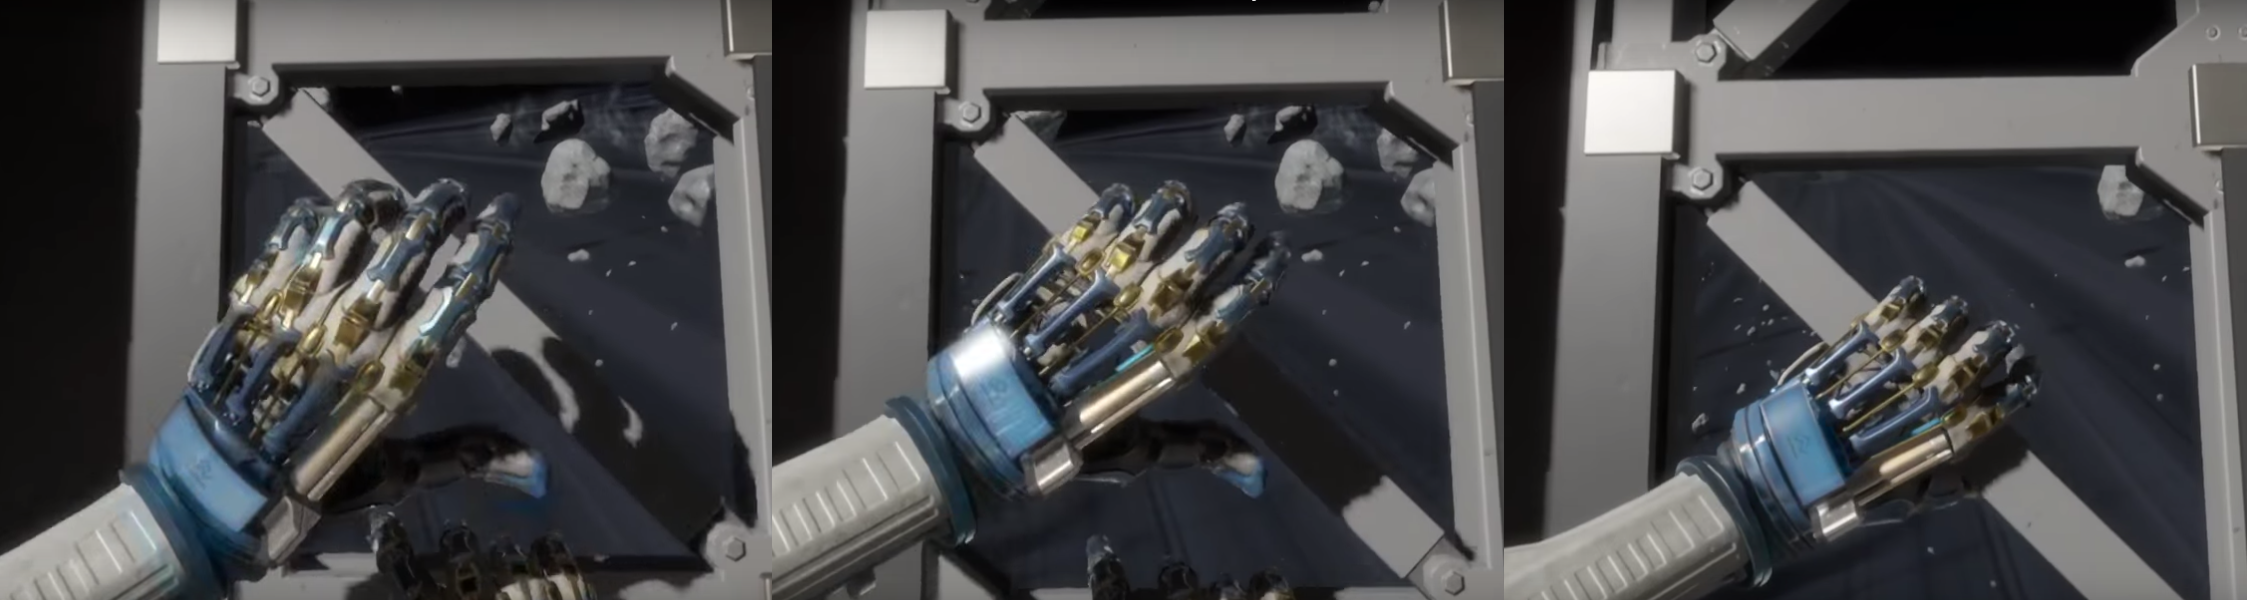
\includegraphics[width=\textwidth]{Sequences/LoneEcho/loneEchoGrip.png}
\caption{Sequence showing the procedural hand posing system in Lone Echo. Captured from video \parencite{loneEchoVideo}. The video can be found here: \url{https://tinyurl.com/loneEchoVideo} .}
\label{fig:loneEchoGrip}
\end{figure}

\section{Research Questions}
\label{sec:researchQuestions}

This work explores ways of dealing with the Virtual Constraints Problem previously described: how can we deal with the conflict between wanting the virtual hands to imitate the user's real hands and at the same time respect the virtual environment?

We consider this problem to be specially prominent in two use cases:

\begin{enumerate}
\item The user places his real hand in a way that would make the corresponding virtual hand be inside of another virtual solid object.
\item The user wants to grab a virtual object but doesn't position the controller and otherwise produce the input that would in a strict simulation allow their virtual hand to lift the object.
\end{enumerate}

These properties should be pursued without losing the degree of control, consistency and intuitiveness that existing unadjusted hand models provide. In sum, the degree of "hand presence" (term commonly used in the VR industry \parencite{Bye2016}) achieved by this model cannot be lost in favor of these goals. The question this work addresses is whether "hand presence" can be improved by dealing with the virtual environment constraints problem.

As secondary objectives, we are interested in finding ways of conveying a sense of the weight of virtual objects when interacting with them and improving the tactility of the virtual hands, improving the feeling of touching virtual objects, which are also aspects currently unsatisfactorily addressed.

Therefore, we are trying to reduce the existing gap between the user's real body and their virtual body and compensate for imprecise user input. In terms of the user's perceptual, sensory experience, it might be possible to improve how hands are controlled in VR.

We focus on experimenting with different ways of adjusting the virtual hands' pose, exploring possible adjusted hand models. We will use the Job Simulator hand model, a great example of an unadjusted hand model, as a reference and baseline to compare our experiments with.

\restoregeometry
\newpage

\chapter{Theoretical Analysis}
\label{chap:theory}
In the previous chapter the terms "immersion", "presence" (and "hand presence") and even "virtual reality" are used in a loose manner. In academia, however, these terms are problematic because of the wide range of fields in which they are used, with very specific and not always similar meanings. Here we will frame the virtual environment constraints problem in existing theories and ground these terms in the academic literature.

\section{Definitions}
\label{sec:definitions}

\subsection{Virtual Reality}
\label{subsec:vrDef}

Virtual Reality is frequently thought of in terms of a collection of hardware commonly associated with the term: head mounted displays, tracking devices, etc... \parencite{Steuer1992} argues that the medium needs a definition with an experiential focus, instead of a technological one, for the purposes of various fields of knowledge such as communication researchers and software developers.

Steuer proposes a definition of Virtual Reality based on the concepts of presence and telepresence. Presence is described by Gibson as "the sense of being in an environment" (cited as found in \parencite{Steuer1992}) and in turn Steuer defines telepresence as "the experience of presence in an environment by means of a communication medium". From these terms we can rewrite Steuer's definition of Virtual Reality as follows:

\begin{displayquote}
\textit{A virtual reality is a real or simulated environment in which a perceiver experiences a sense of being in that environment by means of a communication medium.}
\end{displayquote}

The connection between VR hardware such as the HTC Vive, the Oculus Rift or the PS VR and this concept of virtual reality is, of course then, that these devices amplify user's sense of being in virtual environments.

\subsection{Immersion}
\label{subsec:immersion}

As mentioned before, a term used frequently when talking about the VR medium is immersion. Slater defines immersion as a property useful for the comparison of different virtual reality systems. He borrows the concept of sensorimotor contingencies (SC) from behavioural and brain scientists O'Regan and Noë. SCs are the actions that we know we can perform in order to control our perception: bending down and turning our heads in order to see underneath something and further defines Valid Actions of a virtual reality system as the actions that the user can take that result in changes in perception (sensorimotor actions), or changes to the environment (effectual actions) \parencite{Slater2009}. By Slater's definition:

\begin{displayquote}
\textit{Immersion is a property of the Valid Actions that are possible within a system.}
\end{displayquote}

\subsection{Place Illusion and Plausibility Illusion \textit{in lieu of} Presence}
\label{subsec:PIandPsi}

Slater's definition of immersion focuses on the affordances \parencite{Norman} of virtual reality systems (hardware and software combined) and he builds on it to analyze the concept of presence (in Steuer's terms, telepresence), now focusing on the user experience. He proposes using the terms Place Illusion (PI) and Plausibility Illusion (Psi) instead of it \parencite{Slater2009}:

\begin{displayquote}
\textit{Place Illusion is the illusion of being in a place in spite of the sure knowledge that you are not there. PI is related mainly to the physics of virtual situation. "It is maintained through synchronous correlations between the act of moving an concomitant changes in the images that form perception" Slater explains.}
\end{displayquote}

\begin{displayquote}
\textit{Plausibility Illusion is the illusion that what is apparently happening is really happening in spite of the knowledge that it is not. Psi is determined by the extent to which the system can produce events that directly relate to the user, and the overall credibility of the scenario being depicted in comparison with expectations.}
\end{displayquote}

Slater developed these concepts in his research about why people in virtual reality tend to respond to situations realistically, which is very relevant when considering virtual reality as a tool for therapy for instance. in some cases, this might go further than the goals that game developers have for the experiences they create, since at least to a certain extent, games depict fairly implausible and unrealistic situations.

According to Slater, PI and Psi fuse when we consider the body. We perceive a virtual body to be in the space where we sense ourselves to be (we look down, it seems we are \textit{there}: strong PI), but it is a body that is not ours and over which in principle we have no control, and yet we move our limbs and the virtual body's limbs move in synchrony (an event in the - initially - external world that relates to us: also Psi).

\subsection{Sense of Embodiment}
\label{subsec:embodiment}

The notion of Sense of Embodiment (SoE), proposed in \parencite{Kilteni2012} is perhaps more useful when thinking about virtual bodies:

\begin{displayquote}
\textit{SoE toward a body B is the sense that emerges when B's properties are processed as if they were the properties of one's own biological body.}
\end{displayquote}

Kilteni et al. describe three subcomponents of SoE:

\begin{displayquote}
\begin{itemize}
\item \textit{Sense of Self-Location: one's spacial experience of being inside a body.}
\item \textit{Sense of Agency: "the sense of having global motor control, including the subjective experience of action, control, intention, motor selection and the consious experience of will"} (Blanke and Metzinger's definition, as cited in \parencite{Kilteni2012})\textit{, resulting from the comparison between the predicted sensory consequences of one's actions and the actual sensory consequences.}
\item \textit{Sense of Body Ownership: one's self attribution of the body, implying the sense that the body is the source of the experienced sensations.}
\end{itemize}
\end{displayquote}

\section{TODO}

\begin{itemize}
\item embodied presence \parencite{Schubert1999}
\item reference presence survey \parencite{Schuemie2001}
\item Define virtual reality, presence, immersion and sense of embodiment.
\item Map terms to proposed desirable properties of virtual hands.
\item Survey alternative definitions
\item Fidelity coherence and expectations \parencite{Nowak2003, Argelaguet2016}
\item Why do we care about presence and SoE? -> distinctive quality of the medium, embodied cognition
\item Address Norman's critique of movement based interaction \parencite{Gillies2016}
\item Rubber hand illusion and adjusted hand control model \parencite{Sanchez-Vives2010}, \parencite{Fourneret1998}
\item presence / place illusion / SoE with different sensorimotor contingencies or not in the same capacity as we are present in the real world
\end{itemize}

\restoregeometry
\newpage

\chapter{Methodology}
\label{chap:methodology}
We want some methodology for the experimental and test parts.

\restoregeometry
\newpage

\chapter{Experimental Analysis}
\label{chap:experimentalAnalysis}
This chapter delves into the development of five prototypes, each portraying a different type of behaviour for hands in VR. These different prototypes approach the problem of realism vs sense of embodiment in different ways and to different degrees. In the following sections, we will present a categorization of approaches that can be taken when implementing hands in VR, how our prototypes have been implemented and their pros and cons.\\

All five prototypes have been developed using the Unity engine and the HTC Vive with default controllers for input. The space we've explored during the development of the prototypes have been restricted by these choices. Unity has a set of APIs which we as users of Unity have available to us. These APIs have shaped what has been possible for us during implementation of the prototypes\footnote{Unity's scripting reference is available online \parencite{UnityScriptingReference2017}.}. Furthermore, building the prototypes around using the HTC Vive's controllers as the input method makes our methods and approaches more applicable to hardware that has the same affordances as these. As for the input used to control the hands the position and orientation input is gathered from tracking the controllers and the controllers' trigger buttons are used to indicate how much the fingers should bend, referred to as the closed value (how closed the hand should be)\footnote{The closed value goes from 0 (open) to 1 (closed).}.

These three inputs are the base for different categories of approaches. Each of these inputs can be filtered, by which is meant that the input can be modified or skipped. Filtering on one of the inputs can be seen as using that input as the parameter for a function, which returns a new result. A hand can have a filter for either none of the inputs or one of the inputs or more. Different filtering combinations will give the hand a different behaviour in the virtual world and might result in the hand seeming more realistic when interacting with its environment.

The five hand prototypes are named as follows: \textit{Rigid hand}, \textit{Sliding rigid hand}, \textit{Finger rigid hand}, \textit{Physics hand} and \textit{Rotation hand}. They differ in the way they filter on the player's inputs which gives them a different feel. The detail of which filters and their implementation will be given in the sections below.

\section{Categorization of approaches}
\label{sec:categorizationOfApproaches}
The three player inputs mentioned above (position, orientation and how closed the hand should be) are the base of the categorization of approaches. Each of these inputs can be filtered, by which is meant that the input can be modified or skipped. Filtering on one of the inputs can be seen as using the input as the parameter for a function, which returns a new result which will be used instead of that input. A hand can be implemented with filters on several inputs at once and can have different filters depending on the context. Different filterer combinations will give a different behaviour for the hand in the virtual world and can result in the hand seeming more realistic when interacting with its environment. The hand prototypes will be mentioned in the sections about the three filter variables below, but their implementation will be described in detail in Section \ref{sec:handPrototypes}.

\begin{table}[H]
\centering
\caption{Filter variable combinations.}
\label{tab:filterVariableCombinations}
\begin{tabular}{C{2cm}C{2cm}C{2cm}}
Position & Rotation & Finger position \\ \midrule \midrule
				&					&					\\ \midrule
\Large X	&					&					\\ \midrule
				& \Large X	& 		                \\ \midrule
				&					& \Large X     \\ \midrule
\Large X	& \Large X	&					\\ \midrule
\Large X 	&					& \Large X	\\ \midrule
				& \Large X	& \Large X	\\ \midrule
\Large X 	& \Large X 	& \Large X
\end{tabular}
\end{table}

\subsection{Position filtering}
\label{subsec:categoryPositionFiltering}
A position filter using the definition above is a function, which when enabled, takes the player's positional input from a controller and returns a new value to be used in its stead. This means that the position of the hand in the virtual world will deviate from the controller position.\\

One of our hypotheses is that it's possible to increase the player's sense of embodiment by simulating more realistic behaviour for hands around objects in the world. One of the first steps here is to not allow the hands to penetrate objects. By using position filtering to deviate the hand from the controller position when trying to penetrate an object, the hand can interact more realistically with the world.

The following two figures (Figure \ref{fig:filtersNone} and Figure \ref{fig:filtersPosition}) show an image sequence of a hand with no input filtering and an image sequence with a hand that uses position filtering. The second figure shows the hand stopping when it reaches the object, whereas in the first figure the hand moves through the object.

\begin{figure}[H]
\centering
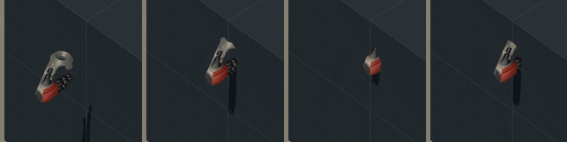
\includegraphics[width=\textwidth]{Sequences/FiltersNone/Seq_FiltersNone.png}
\caption{Sequence showing hand without filters entering obstacle.}
\label{fig:filtersNone}
\end{figure}

\begin{figure}[H]
\centering
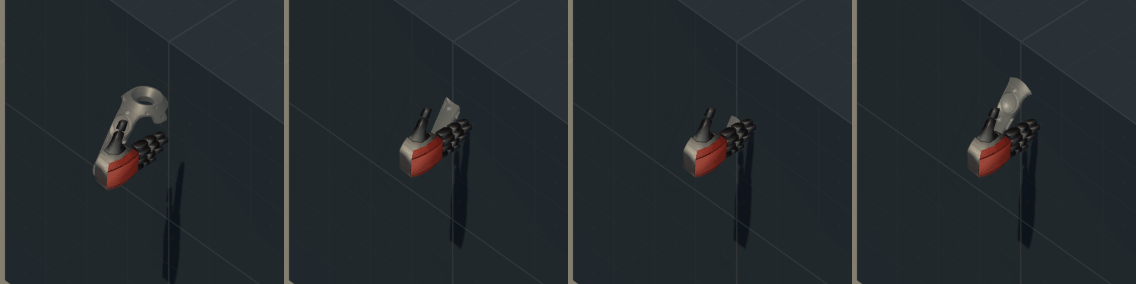
\includegraphics[width=\textwidth]{Sequences/FiltersPosition/Seq_FiltersPosition.png}
\caption{Sequence showing hand filtering on position. Notice that while the hand stays the controller continues to move into the obstacle.}
\label{fig:filtersPosition}
\end{figure}

Implementing position filtering for hands is about determining how to make the hand follow the controller. All of our five prototypes use position filtering, but the implementations of the filters differ. The first distinction is between physics based and non-physics based methods. The Physics hand is the only one of our prototypes that falls into the first category. The way the Physics hand is moved towards the controller is to set the velocity each frame so that the hand will reach the controller within the next frame using the physics system. Using velocities and the physics system to move the hand has several positive aspects. The main gain of using the physics system to move is that it adheres to the rules of the system, including collisions, which means that the hand will not penetrate objects in the world which have colliders. One of the downsides of using the physics system to handle collisions and more is that we as the developers have no direct control over the inner workings of the system and therefore lose some control of how the hand behaves.

As for the prototypes that are implemented using non-physics based methods, their filters are all based on three different approaches to stop the hands from penetrating objects: Sweep and place, skip movement in direction and depenetration. These three methods fall into two categories; pre-collision correction methods and post-collision correction methods. The first two methods fall into the pre-collision correction category, because they try to avoid penetration of objects before it happens, whereas depenetration, which falls into the post-collision correction category will correct the penetration after it has happened. In the different prototypes these three methods are used alone or in combination to create the behaviour wanted from that prototype. The simplest of these prototypes is the Rigid hand. Here only the depenetration comes into play. Depenetrating the hand from an object means to find the direction and distance in which to move the colliders of the hand in order for the hand and the object not to be overlapping anymore. The direction is to the closest point on the object's surface and the distance is the distance needed to move the hand for the hand's colliders to be outside the object's colliders. When moving the hands in this prototype, their position is simply set to the target position on the controller each frame after which they are depenetrated from any objects they would be overlapping with. Since the hand is always depenetrated to the closest surface there is a problem of the hand jumping between surfaces, when the controller is moved around inside static objects. If the hand is closer to surface in one frame and another surface in the next, depenetrating the hand from the object will lead it to move towards the other surface, creating a jump.

The problem of jumping between surfaces, when using depenetration is what the Sliding rigid hand is trying to solve. They employ the other two methods, Sweep and place and skip movement in direction, in order to combat the jumping between surfaces. The main idea behind this prototype is to try avoiding penetrating an object altogether or if it happens to only penetrate a small amount so that depenetrating the hand would always select the same surface from where it entered the object. Sweeping is about taking the hand and calculating how far in a direction it can move before it hits something. Before moving the hand to the controller position we can sweep and see if it would hit an object on the way. If an object was hit then the hand can be placed there instead of placing it at the controller. This way the hand will not penetrate the object although the controller is inside or on the opposite side of it. In Unity sweeping in a direction will not detect an object if the hand already touches the object. Therefore, in subsequent frames from placing the object on the surface, another method is needed for the hand to not penetrate the object. Skipping movement in a direction is one way to alleviate this problem. When the hand is touching the surface of an object, it shouldn't move in the direction towards the surface, because that would lead the hand to penetrate the object. Therefore, we skip all movement along that direction, essentially allowing the hand to only move on a plane. Moving on a plane works wonders, when interacting with cubes, but has its downsides, when dealing with objects with other shapes. Sliding on a plane might lead the hand to penetrate parts of an object that point out or penetrate other objects. Depenetration helps correct the hands in the situations, where they end up inside an object because correcting in one way leads to errors some place else. These three methods combined should lead to hands that don't penetrate objects, but also doesn't jump between surfaces due to depenetration.

The two remaining prototypes, the Finger rigid hand and the Rotation hand, both use the methods mentioned above to achieve their position filtering. The Finger rigid hand use the exact same position filtering method as the Rigid hands and the Rotation hand use a filter similar to the Sliding rigid hand with the exception that it doesn't do any depenetration.

\subsection{Rotation filtering}
\label{subsec:categoryRotationFiltering}
To use a rotation filter is to deviate the hands rotation from the current orientation of the controller. In certain contexts it can be beneficial to filter on rotation for the hand to seem more alive and realistic. Hands can adapt their rotation in several ways and different approaches might be taken depending on the context. When approaching a wall with their hand a player's intention in the real world might be to place their hand flat on the wall (palm first). This behaviour, where the rotation is adjusted to make interacting with walls more natural, can be implemented using a rotation filter, which takes effect when the hand is approaching a surface.

Another reason to use rotation filtering would be about avoiding penetration of objects. Besides being an example of how the hands could feel more natural when approaching walls, the reason for rotating the hand to be palm first when getting close to the surface could also be to avoid penetrating the wall. When the hand rotates, the fingers are rotated away from the wall as well, letting the hand get closer to the wall before it starts penetrating it. Using rotation filtering as a means of avoidance also has the goal of reducing the amount of position filtering needed, by allowing the hand to get closer to the controller position, while still being constrained by objects in the world. Rotation filtering is also a big part of pose snapping, which was mentioned Section \ref{sec:stateOfTheArt}. Pose snapping can be used to show available interactions, for instance in Figure \ref{fig:wilsonGrab} from Wilson's Heart, where the hands snap to a pose when they near the suction cups attached to the player's head. Pose snapping of course works much better in unison with both finger position filtering and position filtering.

The first of the two figures below (Figure \ref{fig:filtersRotation}) shows an image sequence of a hand using only rotation filtering and the second figure (Figure \ref{fig:filtersPositionRotation}) shows an image sequence of a hand using both position and rotation filtering where the rotation filtering is implemented as palm-first towards the surface. It should be noticeable that in the first sequence in the last frame, the hand has entered the obstacle. Using rotation filtering allowed the hand to move closer to the surface before it started penetrating it, but it doesn't stop it completely. Combining the rotation filter with a position filter has the effect of completely stopping it from penetrating the obstacle.

\begin{figure}[H]
\centering
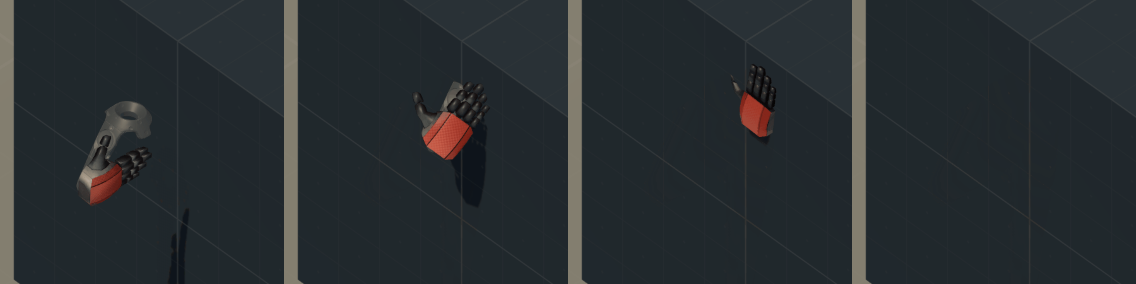
\includegraphics[width=\textwidth]{Sequences/FiltersRotation/Seq_FiltersRotation.png}
\caption{Sequence showing hand filtering on rotation. In the last frame the hand has penetrated the obstacle.}
\label{fig:filtersRotation}
\end{figure}

\begin{figure}[H]
\centering
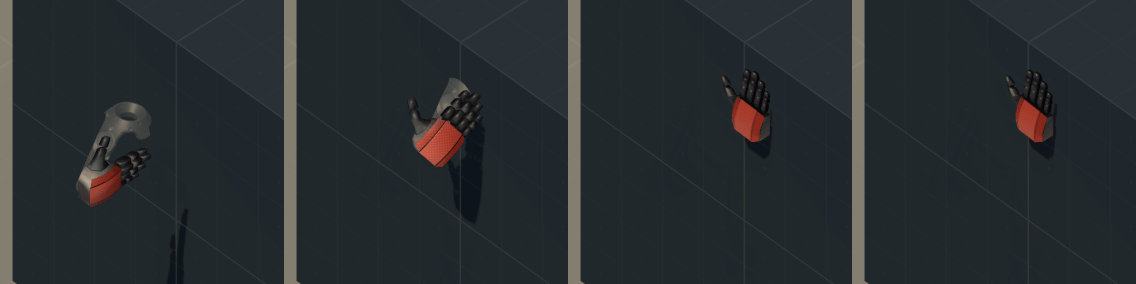
\includegraphics[width=\textwidth]{Sequences/FiltersPositionRotation/Seq_FiltersPositionRotation.png}
\caption{Sequence showing hand filtering on both position and rotation. In the last frame the hand stays on the surface.}
\label{fig:filtersPositionRotation}
\end{figure}

Although all our hand prototypes use position filters, only two of our five hand prototypes (Physics hand and Rotation hand) use rotation filtering.

For the physics hand, we don't use any explicit rotation filtering. The physics system decides the rotation of the hand, when interacting with surfaces. While the controller is within an object, the physics hand can decide to rotate the hand to a flat position (either palm-up or palm-down) in order to reduce the position deviation between the hand and the controller. The rotation happens as a jump and not as a smooth movement towards the surface resulting in a less natural feel during the jump, but a somewhat realistic look afterwards. To improve upon this, explicit rotation filtering could have been added to smoothly rotate the hand to lay flat on the surface, which could remove the jump altogether, but at the same time introduce complexity to the implementation.

Contrary to the Physics hand, the Rotation hand uses explicit rotation filtering. The goal of the rotation filtering for this hand was to always approach a surface palm-first. The main example to explain this choice is the approach of a hand towards a wall. When a player wants to put their hand on a wall, which way would they want to do this? Having an open hand and moving the hand fingers first wouldn't make much sense. It would not give support if the reason for touching the wall was to lean against it, for instance. Rotating the hand so that the palm would be placed firmly on the surface of the wall would make more sense in this case. With this as the main idea behind the rotation, the implementation then had to support this in several cases. The easy case is when the player approaches the wall with an open hand and the palm being closer to the surface than the back of the hand. Depending on the distance to the surface we rotate the palm of the hand the rest of the way until it is directly facing the surface. Another case is what to do when the hand is closed into a fist. In this case, the player is probably trying to punch the wall, which means that the palm shouldn't be facing the wall. Testing for this case isn't necessarily hard in itself, but other cases pile on top of this, including what to do when approaching with the back of the hand, what to do when the player is rotating while the hand is touching the surface and more.

\subsection{Finger position filtering}
\label{subsec:categoryFingerFiltering}
Above is mentioned that the player can control the fingers of the hand by pressing the trigger button on the controller. The hand prototypes all have animations that allow them to be either open or closed into a fist. When filtering on the finger positions the target positions of the fingers, or where we want to place the fingers, deviates from the location indicated by the closed value of the hand.

There are two main reasons for wanting to filter the finger positions. The first reason is relatable to the reason to filter on position; we want the fingers and the hand in general to avoid penetrating objects. By bending the fingers when approaching a surface of an object the hand can move closer to the surface before it starts penetrating, for instance, which reduces how much position filtering is needed. Furthermore, the fingers might also bend individually, which is especially noticeable around edges of objects. Our Finger rigid hand and Rotation hand uses finger position filtering to avoid penetrating objects. The other reason for wanting to filter on finger positions is about indicating whether an object hovered over is interactive or not. In Job Simulator, the fingers bend slightly when the hand is within range of an object that can be grabbed, but they all bend the same amount, though, making the hand look quite robotic. The fingers can of course be filtered individually, which can put the hand in a pose that looks like the hand could be stroking the surface or getting a grip the object. Moving the fingers individually makes the hand look much more realistic in its interaction with objects. This approach has been explored with the Physics hand, which filters on finger positions to show when the hand is hovering over a grabbable object\footnote{A grabbable object is an object which has our grabbable component attached to it. The grabbable component will be described in further detail in section \ref{sec:grabbingSystem} about our grabbing systems.} and is close enough to grab it as well. Furthermore, by bending the fingers towards the surface of the grabbable object when approaching it, the Physics hand allows the player to do things like petting or stroking across object surfaces in a way that looks more natural than with a completely open hand.

\todo[inline]{Perhaps add an image showing the stroking of an object without finger filtering (with open hand) and with the Physics hand finger filtering? The Physics hand's fingers look a lot more natural and less robotic and stiff than without finger position filtering.}

\begin{figure}[H]
\centering
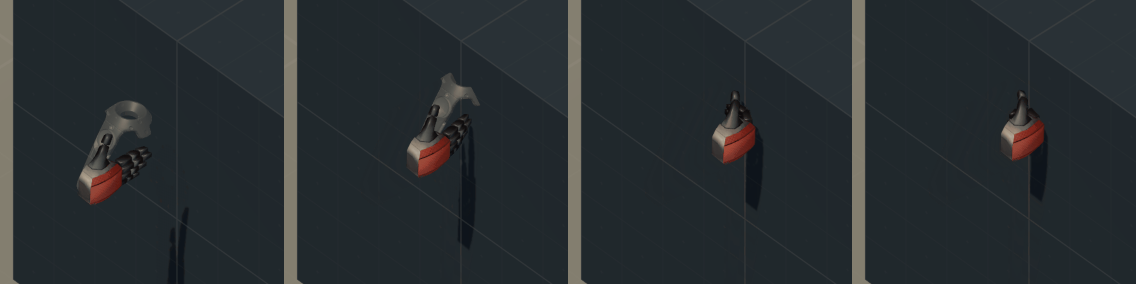
\includegraphics[width=\textwidth]{Sequences/FiltersPositionFingers/Seq_FiltersPositionFingers.png}
\caption{Sequence showing hand filtering on both position and fingers.}
\label{fig:filtersPositionFingers}
\end{figure}

The three hand prototypes that implement finger filtering (the Finger rigid hand, the Physics hand and the Rotation hand) do so in two different ways. The method used for the Finger rigid hand tries to find a suitable closed value for each finger. Each finger can then be animated using this value and its corresponding animation mask. Animation masks are used to isolate a part of the animation data, which makes it possible to use the same animation as for the other hands, while being able to animate each finger individually. The other two hand prototypes make use of an inverse kinematics system (or IK system). Inverse kinematics make use of the kinematics equations to calculate positions for a joint system where we have desired positions for the end effectors. This maps nicely to the movement of fingers, since a finger is a system of joints, where we know the root position of the finger and we'll set the desired location of the end effector, the tip of the finger. The IK system can then calculate how to bend each of the finger's joints to make the tip reach the desired position. To make sure the fingers bend naturally, restrictions can be set for how the joints can bend. The IK system will try to get the tip of the finger's as close to their desired locations without compromising the restrictions for the joints. The restrictions are set up in such a way that the joints can only bend around a single axis which means that they cannot bend sideways, for instance. The axis around which they bend is chosen such that bending the fingers closes the hand into a fist. All fingers bend around the same axis, except for the thumb, because of its placement on the hand. We have used a Unity asset pack called Final IK \parencite{RootMotion2017}, which implements several components and methods that can be used to setup and run IK calculations. To move the fingers using the IK system, we move the IK targets, which are the desired locations for the fingertips.

Without going into too much detail about the implementation of the prototypes before Section \ref{sec:handPrototypes}, it's worth mentioning that finding the adjusted closed value for the fingers in the first method and the position for the IK targets in the second involves depenetration of either the hand as a whole or depenetration of individual fingers as well as raycasting to the surface of nearby objects to find locations to place the IK targets and more.

\section{The hand prototypes}
\label{sec:handPrototypes}
This section will go into depth about how each of the five hand prototypes have been implemented, mention the pros and cons of the different approaches and finally a step-by-step process for creating the behaviour of the prototype will be presented. The table below (\ref{tab:handPrototypes}) stands as a reminder of what filters each of the hand prototypes implements.

\begin{table}[H]
\centering
\caption{The hand prototypes and their filters.}
\label{tab:handPrototypes}
\begin{tabular}{C{2.8cm}|C{2cm}C{2cm}C{2cm}C{2cm}C{2cm}}
 & Rigid hand & Sliding rigid hand & Finger rigid hand & Physics hand & Rotation hand \\ \midrule
Position filter & \Large X & \Large X & \Large X & \Large X & \Large X\\ \midrule
Rotation filter & & & & \Large X & \Large X \\ \midrule
Finger position filter & & & \Large X & \Large X & \Large X 
\end{tabular}
\end{table}

The hands all have a couple of things in common. First the hands require that colliders are set up for their models. We use one box collider for the palm of the hand and one for each part of the fingers, except for the Rotation hand, which only has colliders on the fingertips and the palm. It's important to make sure that the colliders are not able to collide and interact with each other. In Unity we made all game objects in the hand reside on the same layer (but not the default layer) and made the physics system ignore interactions between objects within that layer. If this is not done, the hand might collide with itself and disallow fingers from bending etc. For the physics hands this is taken one step further where each hand, left and right, has their own layer. The second thing we've used for all hands is Unity's rigidbody component. This component lets the hands interact with the world through the physics system. In Unity a rigidbody component can be kinematic or non-kinematic. A kinematic rigidbody is not affected by outside sources which means it's not affected collisions by, for instance. A non-kinematic rigidbody is affected by outside sources and will be affected by, for instance, gravity and collisions. All of our hands use kinematic rigidbodies with the exception of the physics hands. The last thing the hands all need is an animation to close the hand. Our animations consist of two frames; one where the hand is fully open and one where the hand is closed. We can blend between the two frames using the trigger value from the controller, which therefore controls how closed the hand is. Some of the hands have different considerations whether the hand is open or closed. For all hands we consider the hand closed, when the trigger value - which can be between 0 (not pressed) and 1 (fully pressed) - is equal to or greater than 0.5.

Another thing worth mentioning before continuing to the implementation details for each of the hand prototypes is what the target position and rotation of the hand is. The placement of the hand compared to the controller is a decision that impacts how the user will move the controller around to interact with objects and how the hand feels to use. We chose to place the hand compared to the controller in the virtual world in the same way the user's real hand is placed according to the controller in the real world. As shown in Figure \ref{fig:handControllerPlacement}, the right hand is placed to the right of the controller in a position that could grab and hold the controller. The left hand goes on the left side of the controller but is otherwise the same as the right hand. Our reasoning behind this choice was to map the hand as closely to the position of the user's hands in the real world. From now on, when the controller's position and orientation is mentioned, it's the position and orientation the hands display in this image that we're referring to.

\begin{figure}[h]
\centering
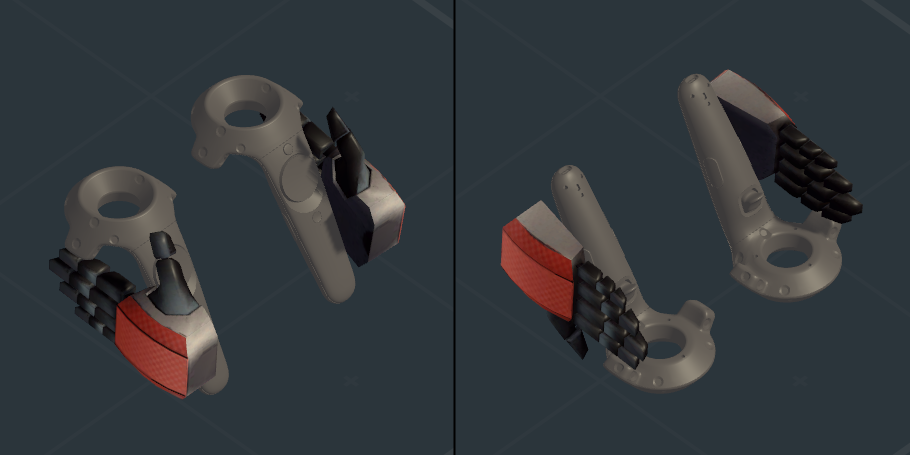
\includegraphics[width=0.85\textwidth]{HandControllerPlacementBoth.png}
\caption{Two images showing the placement of the hands compared to the controllers.}
\label{fig:handControllerPlacement}
\end{figure}

\todo[inline]{Perhaps add a diagram over the hand and its setup, like which parts it consists of, where the origin of the hand is and such.}

\subsection{The Rigid hand}
\label{subsec:rigidHand}
As mentioned above in section \ref{subsec:categoryPositionFiltering}, the Rigid hand moves by setting the rigidbody's position and rotation to the selected position and rotation on the controller. This is done using the $Rigidbody.MovePosition$ and $Rigidbody.MoveRotation$ methods exposed by Unity. Using these methods instead of setting the position and rotation properties directly ensures a smooth rendering in intermediate render frames in Unity and is recommended, when moving a rigidbody, which shouldn't "teleport" \parencite{UnityMovePosition2017}. In the case of moving the hand freely around without any collisions occurring the hand just follows the controller. In the case where the hand has penetrated one or more objects we will depenetrate it from the object. To detect if the hand needs to be depenetrated, we need to check if there is an overlap between the hand's colliders and any other colliders in the world. To reduce the number of colliders to check, we first find all colliders within a radius of the hand. Having these colliders we can now check if any of the hand's colliders have penetrated one or more of them. Unity's Physics API allows us to compute the penetration\footnote{To compute the penetration we use Unity's $Physics.ComputePenetration$ method.} between two colliders, which gives us the depenetration distance and direction. The direction is towards the closest point on the surface of the object penetrated. Iterating over all colliders in both the hand and the penetrated object, we can use the information gathered to move the hand out of the object, correcting the penetration error. The moving and rotation of the hand happens in Unity's fixed update step, which happens at a fixed interval and before the physics simulations. The depenetration of the hand happens in the update step, which happens after the physics simulation. This allows the physics simulation to act upon the situation, where the hand is inside a dynamic object and push it away from the hand. Even though the Rigid hand is kinematic and is not influenced by outside forces, the dynamic objects are and will therefore try to move out of situations, where their collider overlap with others'.

\begin{figure}[H]
\centering
\small
\begin{enumerate}[noitemsep]
\item Move the hand's rigidbody to the target controller.
\item Orient the hand's rigidbody compared to the target controller.
\item Find all colliders within a small radius of the hand.
\item Compute if any of the found colliders are penetrated by one of the hand's colliders.
\item Depenetrate the hand based on the penetration information computed in the previous step.
\end{enumerate}
\caption{Step-by-step process for placing the Rigid hand.}
\label{fig:stepByStepRigidHand}
\end{figure}

The Rigid hand's benefits lie in its simplicity. Very few things are happening, resulting in a simple but suboptimal solution. No matter the orientation of the hand or the position of its fingers, the hand as a whole is moved outside of any penetrated objects so that it is just touching the surface. This makes for a very stiff and lifeless look, when the hand is moved over a surface. Furthermore, as mentioned above, the compute penetration method returns the direction towards the closest point on the surface, but not necessarily a point on the same side of the object as where the hand entered the object. This leads to the hand jumping between different sides of for instance a cube, when the controller is moved between points that are closer to different surfaces. Other drawbacks are linked to the use of a kinematic rigidbody. Using a kinematic rigidbody means that outside forces do not affect the Rigid hand. Besides having to do collision checking manually, which the depenetration is used for, it has implications for things like pushing objects and is especially noticeable when pushing dynamic objects into immovable objects, which will react in a very unstable and jumpy fashion, because they are locked between two objects which aren't affected by physics. Pushing objects will also give no feeling of mass without additional implementations. Usually the mass of the object pushed would be used to create an opposite force enacted upon the hand, giving different masses a different feel. But since the hand doesn't react to outside forces, this difference is not felt.

The Rigid hand is used as the base for the Sliding rigid hand and the Finger rigid hand, which both explore additional filtering to improve the overall feel of the hand. The Sliding rigid hand tries to do away with the jumping between surfaces occurring due the compute penetration method always returning the direction to the closest point on the closest surface and the Finger rigid hand implements finger filtering to reduce the amount of position filtering needed by allowing the hand to move closer to the surface by bending the fingers.

\subsection{The Sliding rigid hand}
\label{subsec:slidingRigidHand}
The Sliding rigid hand is state based with two different states: Outside and touching. The two states let the hand behave differently and are used in different contexts. In each frame one of these states will be executed. The state which will be executed will be determined in the beginning of the frame depending on information from the last state executed and from the current context.

\todo[inline]{Explain what a frame is. Perhaps in a footnote.}

The outside state is executed, when the hand is not touching an object. When executed the hand is first rotated to the orientation of the controller target. After rotating the hand, we sweep towards the controller, checking if there's any object in between the hand and the controller. If no obstacle was in the way, the hand is moved towards the controller. If an object is blocking the path we then position the hand so that it is touching the object. Unity's $Rigidbody.SweepTest$ method gives us the necessary information to do so: direction and distance to the object that was blocking the path\footnote{The direction and distance found by the $SweepTest$ method is between the closest points between the two objects: The direction and distance between the point on the hand that is closest to the closest point on the object hit.}.

There is only one transition from the outside state to the touching state; if the sweep detected an object in between the hand and the controller, while executing the outside state, the hand will have been placed on the surface of the object. In this case we will switch to the touching state. If nothing was obstructing the path the hand stays in the outside state.

As with the outside state, the first thing that happens in the touching state is that we rotate the hand so that it matches the orientation target on the controller. Because we rotated the hand while it was touching an object, we need to check two things; if the rotation has resulted in the hand having penetrated the object or if the rotation has caused the hand to be removed from touching the surface of the object. First, we check if the hand is inside an obstacle and depenetrates it if necessary. This is done in the same fashion as mentioned for the Rigid hand (Section \ref{subsec:rigidHand}). If the hand wasn't inside any object we try to sweep towards the controller position to check if the hand is currently not touching any object. If the sweep resulted in hitting an object in the path towards the controller, we move towards the location hit on that object. This works like mentioned in the outside state above with one small addition. We need to save the normal of the point where the hand touches the surface. When we use Unity's $Rigidbody.SweepTest$ method we gain some information about the object hit, if any. This includes the normal of the point on the object hit by the sweep. We need this normal for the next part: Sliding. Sliding is where we skip movement in a particular direction (and its opposite), effectively moving the hand on a plane. In this case, we skip movement along the normal and its opposite. An example of sliding in use is when the hand is interacting with a flat surface and the controller is inside the surface. When moving the controller around inside, the hand should slide on the plane created by the normal of the contact point, which is approximately the same as sliding across the surface, if the contact point is updated frequently. To implement the sliding we first find the vector between the hand and the target on the controller. This vector is projected onto the plane created with the normal. Moving the hand along this new projected vector reduces the distance to the controller without penetrating the object. As a final step for the touching state, the hand is depenetrated again to make sure it's not inside an object after sliding. To summarize, the touching state rotates the hand and then checks if the hand has now been removed from or placed inside an object and if it has, it's moved to the position where it's touching again. Afterwards the hand then slides to the position on the plane created by the normal which is the closest to the controller.

There are two transitions from the touching state back to the open state. The first transition checks if the controller has moved back outside the object compared to the surface the hand is currently touching. The direction from the hand's current position to that of the controller is computed. If this direction is in the same general direction as the normal of the surface\footnote{To determine if the direction vector points in the same general direction as the normal, we use the dot product of the two. If the dot product is positive they are pointing in the same general direction.}, it means that the controller was moved back outside the object in the direction from where it entered. In this case the hand goes to the outside state. The other transition checks if we can sweep with the hand to the controller. If we can sweep all the way without hitting any objects it means that the hand has slid over an edge and the controller is currently free of any objects. Due to how Unity's $Rigidbody.SweepTest$ method is implemented, it's necessary to move the hand slightly away from the object's surface when sweeping. This is due to the fact that when the object is touched, sweeping doesn't recognize the object being hit. We therefore move the hand slightly back in the direction of the normal of the contact point, before sweeping, but reset the position again when the sweep has been performed. In the case we hit something, the hand is still touching a surface and we stay in the touching state. If not the hand transitions into the outside state.

\begin{figure}[H]
\small
\begin{enumerate}
\item Transition to new state, if necessary.
\begin{enumerate}[noitemsep,label=\alph*.]
\item If the last state executed was outside, transition to the touching state if:
\begin{enumerate}[noitemsep,label=\arabic*.]
\item the sweep during the last outside state execution hit an object.
\end{enumerate}
\item If the last state executed was touching, transition to the outside state if:
\begin{enumerate}[noitemsep,label=\arabic*.]
\item the controller was moved away from the currently touched surface (in the general direction of the normal of the contact point), or
\item the sweeping towards the controller didn't hit any object.
\end{enumerate}
\end{enumerate}
\item Execute selected state behaviour.
\end{enumerate}
% first column
\begin{minipage}[t]{0.49\textwidth}
\small
The outside state:
\begin{enumerate}[noitemsep]
\item Orient the hand's rigidbody compared to the target controller.
\item Sweep towards the target controller.
\item If no obstacles in the path between the hand and the controller, move the hand's rigidbody to the target controller.
\item Else move to the position where the sweep hit the obstacle.
\end{enumerate}
\end{minipage}
\hspace{2em}% <---- Don't forget this %
%second column
\begin{minipage}[t]{0.49\textwidth}
\small
The touching state:
\begin{enumerate}[noitemsep]
\item Orient the hand's rigidbody compared to the target controller.
\item Check if inside object and depenetrate if so.
\item If the hand was not inside an object, sweep towards the target controller.
\item If the sweep hit an object, the controller was not touching. Position the hand on the object hit using the sweep information.
\item Use the normal of the contact point to define a plane on which to slide to minimize the distance to the controller.
\item Check if sliding the hand has led it to penetrating an object and depenetrate if so.
\end{enumerate}
\end{minipage}
\caption{Step-by-step process for placing the Sliding rigid hand.}
\label{fig:stepByStepSlidingRigidHand}
\end{figure}

\todo[inline]{Maybe split the sliding rigid hand step-by-step figure into two figures, so it can be split over two pages.}

What the Sliding hand tries to solve, using the above described state based approach is to remove the jumping created by using only depenetration. This flaw is very evident with the Rigid hand, as the controller moves around inside objects. Since depenetration always moves the hand to the closest point on the surface of the object it's depenetrating from, the main idea of the Sliding rigid hand is to never allow the hand to penetrate deeply enough to select another surface than the one it entered from. This means that unlike the Rigid hand, where the position is updated every frame to the controller target, we always sweep and place, while in the open state, which disallows penetration altogether. Therefore the touching state is the only place where the hand can move or rotate into a position, where it penetrates an object. But because of the restriction of movement along the normal of the contact point, the hand never penetrates the object very far, resulting in the depenetration selecting the same surface even though the controller might be closer to another.

This approach works extremely well on flat surfaces, where the plane created by the normal will be approximately the same as the actual surface the hand is touching, but difficulties arise with non-flat surfaces like curved, rough and concave shapes. Depending on how often the normal is updated, the plane defined by it isn't a very good approximation of the surface, which can lead the hand to not stick to the surface, when moving across it. In our implementation, the normal is only updated upon sweeping, which happens in both states, but only when the hand has been found to be outside the object. The information gathered during depenetration doesn't help much, since the methods for computing the penetration in Unity doesn't give any information about the normal of point of the surface to which the hand would depenetrate, which puts us in a position, where we don't update the normal often enough to handle situations like curved shapes properly. This could be improved upon by finding ways to reliably update the normal of the current contact point more often, which could include sweeping every frame to find the normal during the touching state, for instance. Besides these problems, the same troubles concerning the kinematic rigidbody are inherited from the Rigid hand, leaving us with a hand that works quite well in a low number of situations, which restricts the use cases in which the Sliding rigid hand would perform satisfactory.

\subsection{The Finger rigid hand}
\label{subsec:fingerRigidHand}
The Finger rigid hands are based upon the Rigid hand's way of moving and rotating, but tries to improve upon it by adding finger filtering on top. Where the Rigid hand moves and rotates using the rigibody's $MovePosition$ and $MoveRotation$ methods and then depenetrates the hand from possible overlaps with objects in the world, the Finger rigid hand adjusts the fingers in between the placement and the depenetration.

Before continuing with how the Finger rigid hand and its fingers are placed, we need to mention that the animation for this hand is a bit different from the other prototypes. The animation for the Finger rigid hand has a mask for each finger, which means that the fingers can be animated individually even though we use the same animation frames as for the other prototypes, namely one open and one closed hand frame.

As mentioned above the first thing the Finger rigid hand does is to move to the location of the orientation of the controller by using its rigidbody's $MovePosition$ and $MoveRotation$. When the hand has been placed we save the current closed value of each finger. The closed value here isn't necessarily the same as the trigger button value\footnote{As mentioned above, the trigger button on the controller is mapped to the closing of the hand, by using its value to blend between the open and closed animation frames.}, as this is how closed the finger was after the adjustment last frame. After saving the closed values all the fingers are opened fully using the animation. We need to do this before the next step, which is to calculate the average up vector of all the finger parts for each finger. So for each finger, the average over all its parts' up vectors is saved. When the averages have been calculated, we reset the fingers' closed value to the value saved before and the finger positions are updated according to their closed value using the animation. The next step is to depenetrate the hand from any nearby objects, which is done as previously described. This step is important because we're going to raycast from the fingers later and we need to make sure the origin of the raycasts aren't inside any objects we would like to raycast towards\footnote{In Unity raycasts don't hit backfaces of object models, so to be sure that the raycast hits the object at the correct position, the origin needs to be outside of the object.}. 

With all this legwork done, we're now set to start adjusting the fingers. The general idea is that we want to find out how the fingers are oriented according to the surface they are interacting with. There are three cases we consider for each finger: If the hand is not near any objects, the finger doesn't adjust, if the hand is positioned such that bending the finger will not allow it to move away from the surface (the rotation axis is parallel to the surface normal), we skip adjusting the finger and the last case is if the rotation axis is not parallel with the surface normal. In this case we use the difference between the normal and the rotation axis to decide on how to adjust the finger.

Before we go into the calculations for the individual fingers we first calculate the distance between the hand and the controller. All the fingers use this value to calculate with how much to adjust. With the distance calculated the next steps are performed per finger. To find out if a finger's rotation axis is parallel with the surface normal, we first find the colliders within a radius of the hand\footnote{Unity's physics API exposes the method $Physics.OverlapSphere$ for finding all colliders within a certain radius from a point.} and find the one closest to the finger. If no collider was found near the hand, we skip the finger adjustment and lerp its closed value towards the value determined by the players input. If a collider was found, we use raycasting to find the normal of the closest point on the collider\footnote{The closest point on a collider can be found using Unity's $Collider.ClosestPoint$ method.}. Since we defined the rotation axis of the finger ourselves and we found the normal of the surface, we can take the dot product of the two to see if they are parallel with each other. If they are, the finger cannot bend away from the surface and like with the case of no nearby colliders the finger's closed value is lerped towards the closed value defined by the player's input. In the final case where the normal and the finger's rotation axis are not parallel, we use the dot product between the normal and the average up vector we calculated earlier and the distance from the hand to the controller to find the value with which to adjust the finger's closed value by. We don't use these two values directly, but feed them each to one of Unity's animation curves\footnote{Unity's animation curves are functions that can be visually defined and takes an input value and returns an output value.}: One that evaluates the distance and one that evaluates the dot product. The two resulting values are then multiplied with each other, giving us the adjustment for the finger. After calculating the adjustment value for the finger, we set the finger's closed value equal to the sum of the closed value defined by the player's input and the adjustment value. When all the fingers' closed values have been set, they - along with the animation masks - are used to update the animation of the hand.

As the final thing after having adjusted the fingers, we again want to move the hand to the controller's position\footnote{We only need to move the hand, not rotate it, because depenetrating the hand doesn't rotate it.} and then depenetrate a final time. The reason to this is because having depenetrated and adjusted the fingers might lead to the hand not being positioned at the controller while also not touching the surface of an object. The hand should only be separated from the controller's position, when the hand can't reach it because there's an object in the way. By moving once more and depenetrating we make sure that the hand is placed at either the controller's position or on the surface of the object the controller is inside.

\begin{figure}[H]
\centering
\small
\begin{enumerate}[noitemsep]
\item Move the hand's rigidbody to the target controller.
\item Orient the hand's rigidbody compared to the target controller.
\item Find the average up vector for each finger:
\begin{enumerate}[noitemsep]
\item Open the finger.
\item Take the average of the up vectors of each part of the finger and save it.
\item Move the finger back to the previous position.
\end{enumerate}
\item Depenetrate the hand from any object it might have entered after moving and rotating.
\item Calculate the distance from the hand to the controller.
\item Calculate the adjustment value for each finger and apply it:
\begin{enumerate}[noitemsep]
\item For each finger, find the closest collider within a radius from the hand.
\item If no collider found within range lerp the finger's closed value towards the closed value indicated by the player's input and skip the rest.
\item Find the closest point on the collider found.
\item Find the normal on the closest point of the collider by raycasting to the closest point.
\item If the normal found and the finger's rotation axis are parallel, lerp the finger's closed value towards the closed value indicated by the player's input and skip the rest.
\item Else calculate the dot product between the average up vector of the finger (calculated in one of the previous steps) and the normal.
\item Normalize the distance between the hand and the controller by dividing with a max distance value defined for each finger and clamping the result between 0 and 1.
\item Feed the dot product and the normalized distance into each their animation curve and multiply the results with each other to get the adjustment value for the finger.
\item Set the finger's closed value to the closed value indicated by the player's input summed with the calculated adjustment value.
\item Update the finger's position using each of the finger's closed value and its corresponding animation mask, which allows for animating the fingers individually.
\end{enumerate}
\item Move the hand's rigidbody to the target controller (after depenetration it might have moved away from the controller).
\item Depenetrate the hand after adjusting the fingers and having moved it again.
\end{enumerate}
\caption{Step-by-step process for placing the Finger rigid hand and its fingers.}
\label{fig:stepByStepFingerRigidHand}
\end{figure}

As mentioned above, filtering on finger positions can make the hand feel less stiff, when interacting with objects, but it can also be used with the purpose of avoiding penetration. The main goal of this prototype was to experiment with the latter. As described above, the fingers bend when the hand approaches an object and the direction they bend depends on the hand's angle compared to normal of the nearest point on that object. Bending the fingers like this enables the hand to move in closer to the object, before it needs to filter on the position to avoid penetrating the object. Another benefit from bending the fingers, when interacting with objects is that the hands look a lot less stiff than hands that don't filter on the finger positions, especially because the bending is very smooth. It looks and feels more like a human hand compared to a robotic hand, for instance. The Finger rigid hand doesn't solve any of the problems that the we mentioned about the Rigid hand, of which it is based. The Finger rigid hand still jumps around an object, when moving the controller around inside the object, due to depenetration selecting the closest point on the object to move to and the troubles introduced by using a kinematic rigidbody also still exist. The addition of adjusting the fingers also introduce some new cases where the hands aren't stable. This prototype doesn't handle edges and corners very well. The fingers behave in strange ways since the sweep of the hand still hit the object even though some of the fingers are free to open fully. At corners the hand can't always decide on the side to depenetrate to, because depenetrating to one side, make the fingers bend in a certain way so that when the hand is depenetrated the next time it's closer to another point on the object, resulting in the hand jumping between several positions around the edge or corner. Again, like with the Sliding rigid hand, the Finger rigid hand introduces more problems than it solves, although it proves the fact that the feel of the hand in the cases where it works, is very different from the hands that don't have finger filtering.

\subsection{The Physics hand}
\label{subsec:physicsHand}
The main difference between the Physics hand and the other prototypes is that it is using a non-kinematic rigidbody and is therefore affected by the physics simulation. This means that it can be pushed around by other objects and the physics system will handle collisions. To properly work with the physics system, the hands need to be moved and rotated differently from the other hands. Instead of setting their position and orientation directly, velocities are applied which makes the hand move and rotate to where they need to go. This means that we calculate what velocity is needed for the hand to move the distance between itself and the controller target and the angular velocity needed for the hand to rotate to the controller orientation. In Unity it's important that these velocities are set in the fixed update method, because they need to be applied before the engine's physics calculations takes place\footnote{Unity's order of execution can be seen from a chart in their online documentation \parencite{UnityExecutionOrder2017}.}. Although this is our own implementation it draws heavy inspiration from how the hands are moved in the NewtonVR asset pack \parencite{TomorrowTodayLabs2016}.

Before applying the velocities described above, we adjust the fingers of the hand. As mentioned above, the fingers of the Physics hand are moved using an IK system. The Physics hand has several states that indicate whether the finger positions should be filtered or not. The states are named as follows: Free, Fist, Hover, Holding and Lerp to free. When the hand is not near any objects and the player hasn't closed the hand using the trigger button on the controller the hand will be in the Free state. In this state, the fingers will be positioned according to the animation and the trigger value. The trigger value is used to blend between the open and closed frames of the hand's animation. The animation is used to determine the IK targets' locations. The hand can transition from the Free state into the Fist state, if the player presses the trigger enough for the hand to be considered closed\footnote{As mentioned above, in our prototypes we consider the hand closed when the trigger has been pressed half way, meaning that the trigger value is 0.5 or above.}. In the Fist state the fingers work exactly like in the Free state, dictated by the animation and the trigger value. The reason to have the closed state is to disallow certain transitions that are otherwise possible from the Free state. The Fist state can transition back to the Free state, when the player again opens the hand. Besides transitioning to the Fist state, the Free state can also transition to the Hover state. This happens when there is a grabbable object inside the hand's grab area. The grab area is a trigger collider attached to the hand which indicates the range at which the hand can grab objects in the world. When a grabbable object enters the grab area trigger and the object is below the hand, as in the object is on the side the palm of the hand is facing, the hand enters the Hover state. In the Hover state the finger positions will be filtered in a way that tries to let the fingers approach and touch the object. This filtering will be described further below. From the Hover state the hand can transition to either the Holding state or the Lerp to free state. The Holding state is entered, when the player has grabbed an object. In the Holding state the fingers are not updated, effectively fixating them to their last positions. The hand transitions from the Hover to the Lerp to free state, when there is no grabbable object inside the grab area trigger anymore. The Lerp to free state is inserted in between the Hover and the Free / Fist states to make the transition smooth. In the Lerp to free state the fingers will lerp from their hover positions back to the positions indicated by the animation and trigger button values. When the lerping has finished, the hand will automatically transition to either the Free or the Fist states depending on whether the hand is closed or not. The Free to lerp state can be interrupted if the hand is again hovering over a grabbable object in which case it transitions back to the Hover state.

\missingfigure[figwidth=15cm, figheight=8cm]{Diagram: State change diagram.}

As mentioned above, the fingers positions are only filtered in three of the five states: The Holding state, the Hover state, the Lerp to free state. The Free and Fist states don't filter the input but lets the fingers follow the animation and trigger button value directly. In the Holding state the finger positions are filtered by skipping the input completely. The fingers are fixed, while holding objects. The Hover state is where the most interesting filtering happens. It has several steps to find the positions for the fingers, but first we see if the there is a need to adjust the fingers at all by checking if the grabbable the hand was hovering over is still within the grab area. If not, we skip adjusting the fingers, since in the next frame the hand will transition out of the Hover state, as mentioned above. If there is a grabbable object in the grab area we first place the fingers in accordance to the animation and trigger button value to use as the starting position.

What the Hover state tries to achieve is to find suitable positions on the surface of the grabbable object on where to place the fingers. We try three different methods in priority to find the best location for each finger. The first of the three methods is to find the point on the grabbable that is the closest to the fingertip\footnote{Unity's API allows us to find the closest point on a collider from a given point by using the $Collider.ClosestPoint$ method on the collider in question.}. The next method is to find the point on the surface found by moving along the negative up vector of the fingertip, so finding a point on the object that is directly below the fingertip. For this we use raycasting from the fingertip in the direction of the negative up vector of the fingertip. The final method is to find some direction in between the negative up vector of the fingertip and the direction towards the closest point on the grabbable object. In order to find this middle direction we lerp between the vectors for the direction to the closest point and the negative up vector with respects to a middle interpolation value\footnote{This value is a value between 0 and 1, where 0 returns the start lerping vector and 1 returns the end lerping vector. Using different values moves the position found for the fingers in between the two given direction vectors. We use the value 0.86 for our Physics hand.}. The last two methods are not guaranteed to hit the grabbable object at all. The priority of the three methods is as follows; first we see if moving along the direction which is in between the negative up and the direction to the closest point hits a point on the grabbable object. If it does, we use that point as the position the finger needs to move to. If it didn't hit, we try with the negative up from the fingertip and if it hits, we use that hit point as the position to move the finger to. If none of the above methods resulted in a point on the grabbable object then the closest point on the object is used as the target for the finger. The reason for this prioritization has to do with how good the fingers look after adjusting them for certain placements of the hand compared to the grabbable object and the grabbable object's shape. If the closest point was always used and the hand was hovering over a grabbable cube with the palm on one of the surfaces and the fingers sticking out over the edge, the result would lead to the two furthest joints in the fingers both bending about 90 degrees without the joint between the fingers and the palm bending much, which is not a natural pose and is therefore not ideal (\textbf{\textit{REF: Image about cube example}}). The same will occur when hovering over thin objects like sticks or bats. The closest position on the grabbable from the fingertips will be close to the palm resulting in the weird pose. Using the negative up vector of the fingertips will also not work in a lot of cases. If we again look at the example with the grabbable cube. If the hand is completely open and the fingers are sticking out over the edge, moving along the negative up vector will not lead to a hit on the cube. Because of this, having a middle point between the closest point and the negative up can help in these cases by bending the fingers towards the grabbable object, but with a more natural pose than what results from the closest point. When the positions for the fingertips have been found by using one of these methods we lerp the IK targets of the fingers towards the found positions, as to smooth out the movement, after which we call the IK system to solve for the new position.

\missingfigure[figwidth=15cm]{Diagram: Cube example showing why the middle direction is important.}

\begin{figure}[H]
\centering
\small
% POSITION AND ROTATION.
\begin{flushleft}
Position and rotation:
\end{flushleft}
\begin{enumerate}[noitemsep]
\item Calculate the angular velocity needed to rotate the hand to the orientation of the controller in this frame and apply it to the hand's rigidbody.
\item Calculate the velocity needed to move the hand to the position of the controller in this frame and apply it to the hand's rigidbody.
\end{enumerate}
\caption{Step-by-step process for placing the Physics hand.}
\label{fig:stepByStepPhysicsHandPositionRotation}
\end{figure}

\begin{figure}[H]
\centering
\small
% FINGER POSITIONS.
\begin{flushleft}
Finger positions:
\end{flushleft}
\begin{itemize}[noitemsep]
\item If in the Hover state:
\begin{enumerate}[noitemsep]
\item Check if there is a grabbable object in the grab area of the hand below the palm. If not, skip the rest.
\item Move all fingers to the location indicated by the animation and the trigger button value as a starting position.
\item For each finger, get the negative up vector from the fingertip.
\item Get the closest position from the fingertip to the grabbable object and create a direction vector starting from the fingertip and pointing at the closest point.
\item Calculate the middle vector as a vector which resides between the negative up and the closest point direction. This can be done by lerping. The amount by which to lerp is a variable which needs to be tweaked.
\item Raycast towards the middle direction with the max distance being the radius of the grab area. If the grabbable object was hit, set the hit point as the finger's target.
\item If the previous raycast didn't hit the object, raycast in the negative up direction with the same distance. If the object was hit, set the hit point as the finger's target.
\item If none of the raycasts hit, use the closest point on the grabbable object as the finger's target.
\item Set all fingers to their open position using the animation as a base. This is to start the IK solving from the same location every frame.
\item Lerp the finger's IK targets towards the calculated finger targets.
\item Let the IK system solve for the new IK targets and move the fingers.
\end{enumerate}
\item If in the Lerp to free state:
\begin{enumerate}[noitemsep]
\item For each finger, save its current IK target position.
\item Get the position that each finger would have according the the animation and trigger button value.
\item Find an intermediate position for the fingers slerping\footnote{SOMETHING ABOUT SLERPING HERE!} from the saved IK target position towards the animation position.
\item Set the IK target of the finger to the intermediate position found for it.
\end{enumerate}
\item If in the Holding state:
\begin{enumerate}[noitemsep]
\item Skip all finger movement.
\end{enumerate}
\item All other states:
\begin{enumerate}[noitemsep]
\item Set each finger's IK target to the position indicated by the animation and trigger button values.
\end{enumerate}
\end{itemize}
\caption{Step-by-step process for placing the Physics hand's fingers.}
\label{fig:stepByStepPhysicsHandFingers}
\end{figure}

The previously mentioned prototypes all have troubles caused by using a kinematic rigidbody. Collisions must be handled manually and that creates a lot of cases that need to be solved before the hands look really nice, when interacting with objects of different shapes and types. Unity's physics system already handles most of these cases, when two physics objects interact with each other. Therefore, the main idea behind the Physics hand is to let the physics system handle all the difficulties that arise due to collision handling. But besides handling just collisions, using a non-kinematic rigidbody enables the Physics hand to do a couple of extra things out of the box, which include lifting and having a sense of weight when interacting with objects. Lifting here means to be able to lift an object without grabbing it using a grabbing mechanism\footnote{All hand prototypes implement a grabbing mechanism, which when activated allows the grabbed object to follow the hand. The different implementations are described below in Section \ref{sec:grabbingSystem}.}, which in our case is activated by pressing the trigger until the hand is closed. An example of how to lift an object using the Physics hand is to place the left and right hand on either side of an object, push the hands towards the object and then move the controllers upwards. The physics system will use the friction between the materials, the mass and the force with which the hands push into the object to enable the lifting of the object. This also leads into the sense of weight. Since all interactions, collisions included, are now fully physics based it means that the objects the hands interact with are also applying forces to the hands. When trying to lift a heavy object, the player might not be able to and the hands will slide across the surface instead of lifting the object. The sense of weight also applies to the context of pushing, where the hands will be separated more from the controller position, when pushing heavier objects than with lighter objects, which gives a different feel to pushing objects of different weight.

Besides all these good things that comes with the use of a non-kinematic rigidbody, there are also downsides that tag along. The rotation filtering occurring with the Physics hand is also controlled by the physics system, as with the position filtering, but in some cases it doesn't act in a satisfactory fashion. When placing the hand flat on the surface of an object and then turning the controller, the hand stays flat on the surface, which feels very natural. The opposite of this is when the hand is pushed towards the surface fingers first. At first the hand will look a lot like the Rigid hand, staying outside the object, but when the controller is far enough from the hand, it jumps to a position where the hand is flat on the surface. This jump feels unnatural. One way to avoid this jump would be to create explicit rotation filtering to handle the cases, where the hand would rotate in a frame and smoothly rotate the hand instead. This problem isn't seen very often, though, since the hand rotates more smoothly, when it approaches the surface at an angle instead of straight on. Along with the rotation jump there are also problems that are related to the moving of the fingers. When the fingers are bend they change the shape of the rigidbody, moving the center of mass, which applies forces to the rigidbody (\textbf{\textit{PERHAPS FIND NAME OF THIS CONCEPT OF PHYSICS}}). This means that bending the fingers could result in the hand moving and rotating, because of the applied forces, which is not the wanted behaviour. The hand should be able to stay still, while the fingers are bending. The way we solved this was by increasing the drag and angular drag of the hand's rigidbody to the point where the movement and rotation caused by bending the fingers wasn't noticeable anymore.


\subsection{The Rotation hand}
\label{subsec:rotationHand}
The Rotation hand is the only prototype we implemented that explicitly filters on all three variables: position, rotation and finger positions. It has two modes of movement. First, we check if there are no objects in the hand's vicinity. We can do this by using Unity's physics API which exposes the method $Physics.OverlapSphere$ for finding all colliders within a certain radius from a point. If there are no objects nearby the position and orientation of the hand is set to the position and orientation of the controller. If there are object nearby we act upon the closest collider. We first want to rotate the hand. The goal of the explicit rotation filtering is to make the palm face the surface of the object, when the hand is open and make the front of the hand face the surface, when the hand is closed into a fist (\textbf{\textit{IMAGES HERE?}}). The rotation should be more or less complete depending on the distance to the object meaning that if the hand is touching the object, the palm should be facing directly towards the surface and if the hand is far away it should orient itself like the controller target and blend when in-between (\textbf{\textit{CREATE IMAGE SEQUENCE}}). To begin, the hand's orientation is first set equal to that of the controller target. This is used as the starting position from where we apply additional rotation. To calculate the additional rotation to apply to the hand, when approaching an object, the normal of the object's surface is required. Depending on if the hand is open or closed we also want the palm's up vector or negative forward vector respectively. In the case of the open hand, we want the palm's up vector to rotate towards the normal of the surface, when the distance is reduced. Unity provides a lerp method to linearly interpolate between two vectors\footnote{In Unity the $Vector3.Lerp$ method can be used to linearly interpolate between two vectors.}, which is used to find the direction vector to which the palm's up should point depending on the current distance to the surface. To increase the amount of control we have over the rotation, we don't use the distance directly. We first pass it through a function which we define using one of Unity's animation curves. This way we can control if the hand should rotate faster between certain distances, for instance. When the direction vector has been calculated, we use it together with the current up vector (or negative forward in the case of the hand being closed) to define a rotation\footnote{The rotation between two vectors can be calculated using Unity's $Quaternion.FromToRotation$ method.}, which we add to the hand's current rotation.

When rotation has occurred it's time to move the hand. In order for the hand not to penetrate the object it's moving towards, we sweep from the hand towards the controller position. When sweeping, we don't want the fingers to be taken into account. The accommodate for this, we don't have colliders on the fingers except for the fingertips. These colliders are disabled at all times, except during the calculation of the finger positions, which is described below. As mentioned before, Unity's $Rigidbody.SweepTest$ method doesn't detect objects that the hand is already touching, so we move it back slightly in the direction of the surface normal before sweeping. If the sweep hit an object the hand is moved to the hit position after which its slid across the surface to reduce the distance to the controller position. The sliding works in the same way as for the Sliding rigid hand (Section \ref{subsec:slidingRigidHand}). The normal is used to create a plane upon which the vector which spans between the hand position and the controller position is projected upon. This new vector is then what determines where to move the hand. If no object was hit during the sweep test, the hand is moved straight to the controller position.

The fingers of the Rotation hand are moved using an inverse kinematics. When we want to move the fingers, there are two contexts we consider; either the hand is near objects that the fingers might interact with or it isn't. In both cases we start off by setting the fingers' targets to the positions defined by the controller's trigger value. This position is gathered from the hand animation, which is blended between an open and closed animation frame. In the case that there aren't any nearby objects nothing more is done to the fingers. When the player presses the trigger they will therefore close the hand and it will open, when they release the trigger. In the other case, where the hand is close to one or more objects, the fingers will be adjusted so that they don't penetrate any objects. To do this, all colliders within a radius are found using the same method described above. For each of the found colliders we check if the fingertips are inside by computing the penetration between the fingertip collider and the found collider. Before this step we enable the fingertip colliders, which are normally disabled. After computing the penetration we disable the fingertip collider again. The distance and direction gathered from computing the penetration is then used to move the finger's IK target. This means that the desired location the finger is trying to move to is moved outside of the object.

\begin{figure}[H]
\small
Position and rotation:
\begin{enumerate}[noitemsep]
\item If no objects are within a radius from the hand, move towards the position and the rotation of the controller and skip the rest.
\item Else find the orientation to rotate towards:
\begin{enumerate}[noitemsep]
\item Get the normal of the closest point on the closest object.
\item Get the current palm direction vector as the palm's up vector if the hand is open and the palm's negative forward vector if the hand is closed.
\item Calculate target direction vector by lerping between the current palm direction vector and the normal vector.
\item Calculate the rotation between the current palm direction vector and the target direction vector.
\item Rotate the hand towards the sum of the controller orientation and the rotation calculated in the previous step.
\end{enumerate}
\item And then move the hand:
\begin{enumerate}[noitemsep]
\item Move the hand a tiny bit in the direction of the normal (so the hand is not touching the object, when sweeping).
\item Sweep the hand towards the controller position.
\item If the sweep hit an object, place hand at hit point and slide to minimize the distance between the hand and the controller.
\end{enumerate}
\end{enumerate}
Finger positions:
\begin{enumerate}[noitemsep]
\item Set each finger's IK target to the animation's finger tip position.
\item Find all colliders within a radius from the hand.
\item If no colliders were found, skip the rest.
\item Else enable finger tip colliders.
\item Compute each finger tip collider's penetration with the colliders found in step 2.
\item Move each finger's IK target using the distance and direction found by computing the tip's penetration.
\item Disable the finger tip colliders again.
\end{enumerate}
\caption{Step-by-step process for placing the Rotation hand and its fingers.}
\label{fig:stepByStepRotationHand}
\end{figure}

\begin{itemize}[noitemsep]
\item[GOOD] The palm rotation is quite stable and looks good, but can be improved (like not rotating when approaching with the back of the hand, adding more cases for different behaviour).
\item[BAD] The finger targets don't always depenetrate correctly (they might choose wrong surfaces to depenetrate to).
\item[BAD] Depenetrating the finger targets and placing the fingertip there doesn't mean that the rest of the finger isn't penetrating the object.
\end{itemize}

\todo[inline]{Write a small conclusion for the Rotation hand. This should include what it does well and where it fails. The rotation hand's palm rotation works pretty well, but it could do with some improvements, like not rotating when approaching the wall with the back of the hand (essentially adding more cases for different behaviour). Furthermore, the fingers are not looking too nice and often penetrate the object it's interacting with, since only the finger tips are depenetrated.}

\subsection{Unsolved problems}
\label{subsec:unsolvedProblems}

\todo[inline]{Describe problems that we've identified but aren't solved by any of the hands.}

\begin{itemize}[noitemsep]
\item When hand moves over edge of object that was blocking movement, it jumps/lerps to the controller position. This always looks unrealistic, but we haven't found a good solution.
\end{itemize}

\section{Real hand visualization}
\label{sec:handVisualization}

\todo[inline]{Because the hand separates from the controller, when the controller is put into objects in the virtual world, we decided to implement a wireframe hand representing where the hand would have been, if no filters had been applied to it. This shows the player where there "real world" hand is in the virtual space and also shows that the filtering is intentional and that we still know where their real hand is.}

\section{Rumble}
\label{sec:rumble}

\todo[inline]{The section about rumble is just a short section about how we tried to implement rumble into our demoes and how it didn't work out too well. First off we had too much rumble and on too many things and in the short time we had to try and fix it, we made only slight improvements to that. Perhaps the section will focus more on what rumble can be used for.}

\section{The grabbing system}
\label{sec:grabbingSystem}

\todo[inline]{We've implemented several different types of grabbing, although we ended up using one type for our demoes. The types include: parenting, using a fixed joint and setting velocities (like the way we set the velocities for the Physics hand). These different grabbing types have different pros and cons attached to them. Furthermore, describe our grabbable component, which is used to detect if an object can be grabbed and is also used for finger filtering to show when the hand is hovering close enough to a grabbable object for it to be grabbed.}

\restoregeometry
\newpage

\chapter{Results}
\label{chap:results}

\restoregeometry
\newpage

\chapter{Conclusion}
\label{chap:conclusion}

%\input{somepage.tex}
\restoregeometry
\newpage

\printbibliography

\end{document}